\documentclass{sigchi}

% Use this command to override the default ACM copyright statement (e.g. for preprints). 
% Consult the conference website for the camera-ready copyright statement.


%% EXAMPLE BEGIN -- HOW TO OVERRIDE THE DEFAULT COPYRIGHT STRIP -- (July 22, 2013 - Paul Baumann)
% \toappear{Permission to make digital or hard copies of all or part of this work for personal or classroom use is 	granted without fee provided that copies are not made or distributed for profit or commercial advantage and that copies bear this notice and the full citation on the first page. Copyrights for components of this work owned by others than ACM must be honored. Abstracting with credit is permitted. To copy otherwise, or republish, to post on servers or to redistribute to lists, requires prior specific permission and/or a fee. Request permissions from permissions@acm.org. \\
% {\emph{CHI'14}}, April 26--May 1, 2014, Toronto, Canada. \\
% Copyright \copyright~2014 ACM ISBN/14/04...\$15.00. \\
% DOI string from ACM form confirmation}
%% EXAMPLE END -- HOW TO OVERRIDE THE DEFAULT COPYRIGHT STRIP -- (July 22, 2013 - Paul Baumann)


% Arabic page numbers for submission. 
% Remove this line to eliminate page numbers for the camera ready copy
% \pagenumbering{arabic}
%thanks

% Load basic packages
\usepackage{balance}  % to better equalize the last page
\usepackage{graphics} % for EPS, load graphicx instead
\usepackage{times}    % comment if you want LaTeX's default font
\usepackage{url}      % llt: nicely formatted URLs
\usepackage{makecell}
\usepackage{changepage}
\usepackage{mathtools}

% llt: Define a global style for URLs, rather that the default one
\makeatletter
\def\url@leostyle{%
  \@ifundefined{selectfont}{\def\UrlFont{\sf}}{\def\UrlFont{\small\bf\ttfamily}}}
\makeatother
\urlstyle{leo}


% To make various LaTeX processors do the right thing with page size.
\def\pprw{8.5in}
\def\pprh{11in}
\special{papersize=\pprw,\pprh}
\setlength{\paperwidth}{\pprw}
\setlength{\paperheight}{\pprh}
\setlength{\pdfpagewidth}{\pprw}
\setlength{\pdfpageheight}{\pprh}

% Make sure hyperref comes last of your loaded packages, 
% to give it a fighting chance of not being over-written, 
% since its job is to redefine many LaTeX commands.
\usepackage[pdftex]{hyperref}
\hypersetup{
pdftitle={SIGCHI Conference Proceedings Format},
pdfauthor={LaTeX},
pdfkeywords={SIGCHI, proceedings, archival format},
bookmarksnumbered,
pdfstartview={FitH},
colorlinks,
citecolor=black,
filecolor=black,
linkcolor=black,
urlcolor=black,
breaklinks=true,
}

% create a shortcut to typeset table headings
\newcommand\tabhead[1]{\small\textbf{#1}}


% End of preamble. Here it comes the document.
\begin{document}


\title{User-Defined Game Input \\for Smart Glasses in Public Space}


%\author{\alignauthor Chun-Yen Hsu, Ying-Chao Tung, Han-Yu Wang, \\Silvia Chyou, Jer-Wei Lin, Mike Y. Chen\\
%\affaddr{Mobile and HCI Research Lab, National Taiwan University} \\ 
%\email{\{hcythomas0125,tony61507,huw12313212,silvia.chyou,evin92\}@gmail.com,\\ mikechen@csie.ntu.edu.tw}
%}


\maketitle




\begin{abstract}

Smart glasses, such as Google Glass, provide always-available displays not offered by console and mobile gaming devices, and could potentially offer a pervasive gaming experience. 
However, research on input for games on smart glasses has been constrained by the available sensors to date. 
To help inform design directions, this paper explores user-defined game input for smart glasses beyond the capabilities of current sensors, and focuses on the interaction in public settings. 
We conducted an user-defined input study with 24 participants, each performing 17 common game control tasks using 3 classes of interaction and 2 form factors of smart glasses, for a total of 2448 trials. 
Results show that users significantly preferred non-touch and non-handheld interaction over using handheld input devices, such as in-air gestures. Also, for touch input without handheld devices, users preferred interacting with their palms over wearable devices (51\% vs 20\%). 
In addition, users preferred interactions that are less noticeable due to concerns with social acceptance, and preferred in-air gestures in front of the torso rather than in front of the face (63\% vs 37\%). 

%
%Without a controller or direct-touch, game control on smart glasses differs from existing console and mobile games. Although current game control on smart glasses is explored by developers based on system capability, the control set is not reflective of user behavior. We present a user-defined game control study in public space to collect user behavior without influence from system limitation. In all, 2448 game controls from 24 participants were logged, analyzed, and paired with think-aloud data for 17 commands performed with 3 interaction methods %(\emph{In-Air}, \emph{On-Body} and \emph{Phone}) 
% and 2 different smart glasses  %(\emph{Google Glass} and \emph{Epson BT-100})
% . Our findings indicate that the user preference with \emph{In-Air} interaction is significant higher than \emph{Phone} controller, that users prefer a relatively unobtrusive control area with concerning social acceptance, and that different form factors of smart glasses do influence how users create control actions. We also present a complete user-defined game control set with agreement scores and taxonomy. Our results will help designers create better game controls informed by user behavior.
%

% Game control on smart glasses differs from existing console and mobile games due to the lack of physical game controllers or direct-touch. Although current game control on smart glasses is explored by developers based on system capability, the set of controls is not reflective of user behavior. 
% To create better game control, we presented a user-defined game control study in public space to collect user behavior. In all, 2448 game controls from 24 participants were logged, analyzed, and paired with think-aloud data for 17 commands performed with 3 interaction methods (\emph{In-Air}, \emph{On-Body} and \emph{Phone}), and On-Body method is inclusive of wearble devices' control. The study used 2 different forms of smart glasses (Google Glass and Epson BT-100) and users don't need to consider the system limitation. We find that users prefer using \emph{In-Air} and \emph{On-Body} inputs to perform the game controls in a relatively unobtrusive area, and that different forms of smart glasses do influence how users create control actions. Users will choose less noticeable control methods because of social acceptance. We also present a complete user-defined game control set with agreement scores and taxonomy data. 
% Our results will help designers create better game control based on user behavior.

% Abstract 的 Take home note 不夠明顯
% Abstract 強調 System Limitation 不再考慮範圍內
% Abstract On Body要看出來 Wearble Diveces的操作
% 1.使用者在Public Space Gaming時 比較prefer In-Air 及 On-Body Interaction方式。
% 2.使用者會因為Social Acceptable的原因而選擇較不引人注目的操作方式。
% 3.眼鏡的Form Factor (螢幕大小&位置) 影響了使用者對In-Air Gesture的設計。

\end{abstract}


\keywords{
  Game, input, control, smart glasses, guessability, think-aloud, user-defined, public space, pervasive gaming, wearable.
	% Guides; instructions; author's kit; conference publications;
	% keywords should be separated by a semi-colon. \newline
	% \textcolor{red}{Optional section to be included in your final version, 
 %  but strongly encouraged.}
}

%\category{K.8.0.}{General}Games; {H.5.2.}{Information Interfaces and Presentation}
%: User Interfaces - \emph{Interaction styles, evaluation/methodology, user-centered design.}

% See: \url{http://www.acm.org/about/class/1998/}
% for more information and the full list of ACM classifiers
% and descriptors. \newline
% \textcolor{red}{Optional section to be included in your final version, 
% but strongly encouraged. On the submission page only the classifiers’ 
% letter-number combination will need to be entered.}



\section{Introduction}

%The invention of smart glasses offers more 
%Emerging wearable computing devices atrract extensive attention worldwide. 
Smart glasses provide always-available displays and offer the opportunity for instantly available information and pervasive gaming experiences. 
%We can play a game without any setup, like taking out the mobile phone from the pocket. 
Compared to game consoles and mobile gaming devices, smart glasses do not have touchscreens and currently do not support handheld controllers specifically designed for gaming.
Current smart glasses, such as Google Glass and the Epson Moverio, support input via voice, touchpads, cameras, gyroscopes, accelerometers, and GPS.
Games designed specifically for Google Glass \cite{MiniGames} utilize these sensors as game control. 
% ``Balance'' uses gyroscopes to capture users' head tilt, 
For example, ``Clay Shooter'' utilizes the user's voice to trigger a shotgun, and ``Shape Splitter'' detects in-air gestures via the built-in cameras. 
For the Epson Moverio glasses, wired trackpads are used as handheld controllers.

% Nevertheless, what kinds of control actions do regular users make naturally? In the users' minds, what characteristics are important for such game controls? Will they prefer in-air gestures or just a physical controller? How consistent are game controls employed by different users for the same game task? 
% Although designers may organized their game controls in a principled, logical fashion, user behavior is rarely so systematic. As McNeill \cite{HandAndMind} writes in his laborious study of human discursive gesture, ``Indeed, the important thing about gestures is that they are \emph{not} fixed. They are free and reveal the idiosyncratic imagery of thought''.

 \begin{figure}[!t]
  \centering
  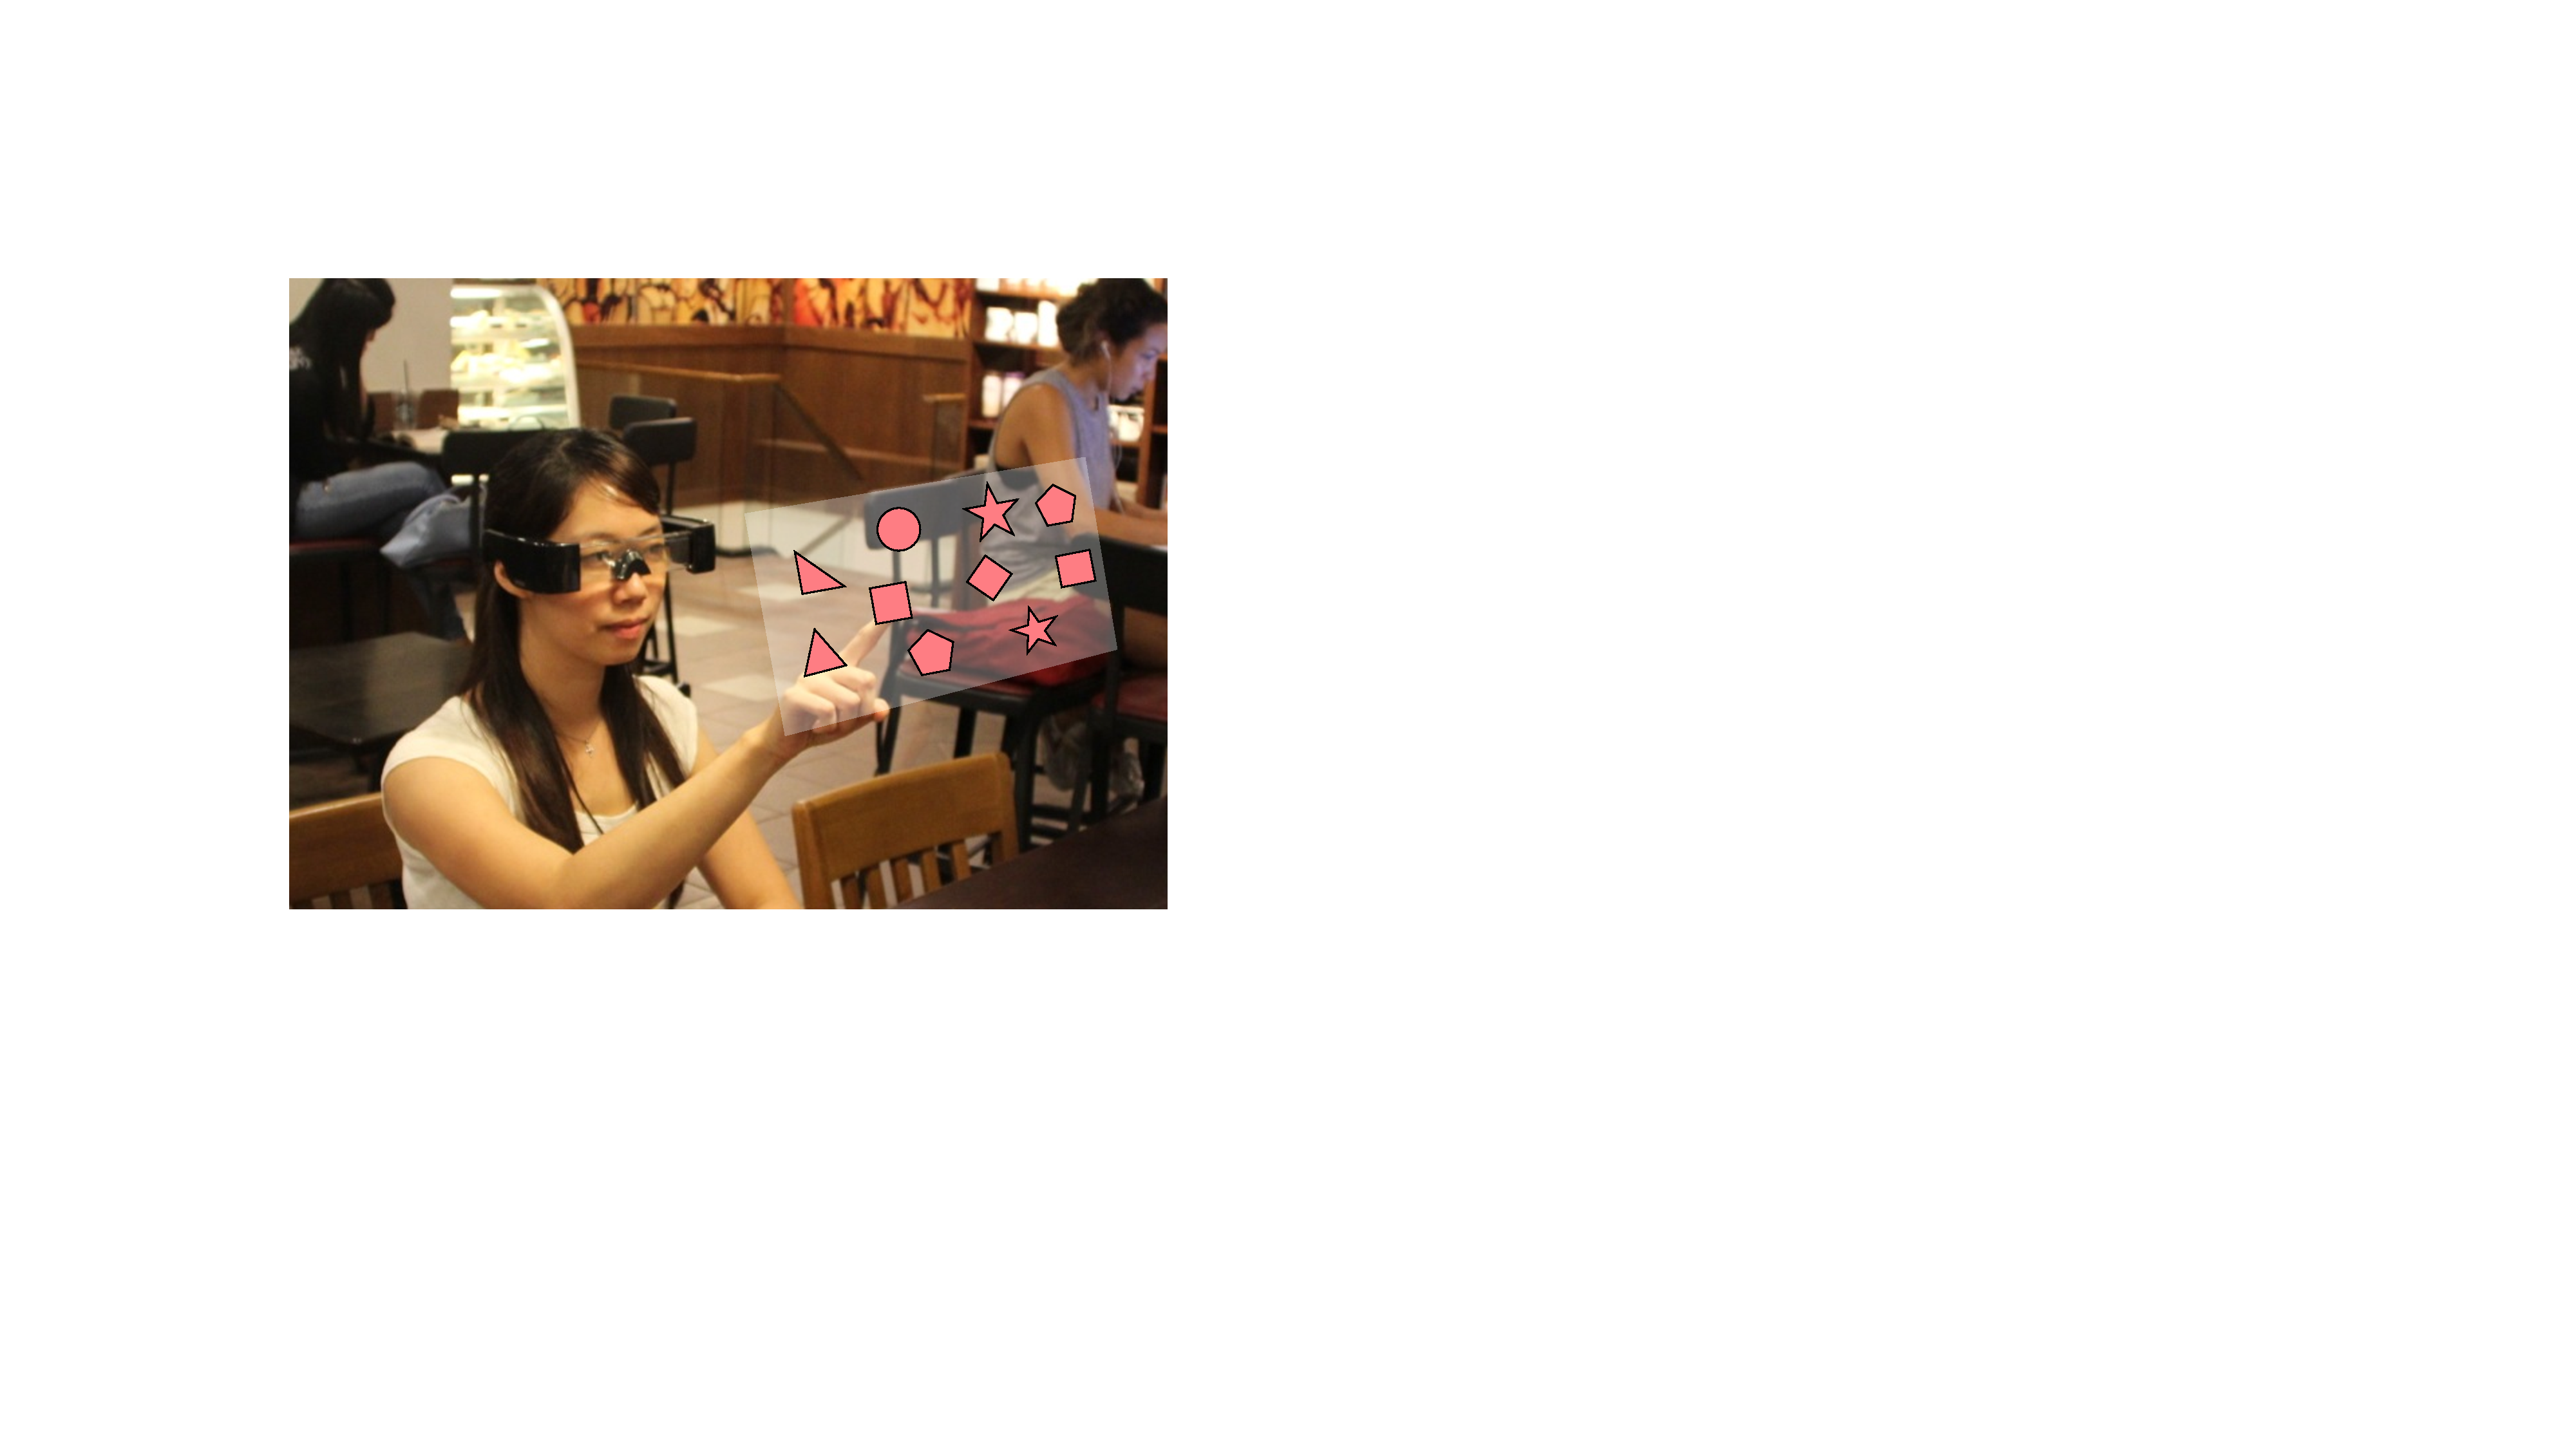
\includegraphics[width=0.8\columnwidth]{TopFigure2.pdf}
  \caption{A study participant performing an in-air gesture to drag an object seen through the immersive smart glasses in a public coffee shop.}
  \label{fig:TopFigure}
  \end{figure} 

To better inform the interaction design of games for smart glasses, we aimed to explore the design space without being constrained by the capabilities of current sensors. We used the guessability study methodology \cite{Wobbrock:2005:MGS:1056808.1057043}, and presented the \emph{effects} of game controls to the participants in a real-world, public environment. We then elicited what the participants felt was the most appropriate \emph{causes} to invoke the corresponding effects. 

For input tasks, we analyzed 90 popular games to identify the game controls used by more than one game, which resulted in a set of 17 tasks. We also explored the form factors of smart glasses displays, and included both types in the study: 1) \emph{immersive}, which displays content spanning users' field of view (e.g. Epson and Sony's smart glasses), and 2) \emph{off-to-the-side}, with displays content in the corners of users' field of view (e.g. Google Glass).

In order to compare different types of interaction while keeping the experiment tractable, we grouped the different types of input into the following 3 classes:
\begin{itemize}
  \item \emph{handheld}: input types that make use of handheld controllers, such as smartphones and the wired trackpads used by Sony's SmartEyeglass and Epson's Moverio glasses.
  \item \emph{touch}: non-handheld touch input, such as gesturing and tapping on body surfaces, and touch-sensing wearable devices (e.g. smart rings, watches, and glasses). These provide tactile feedback.
  \item \emph{non-touch}: non-handheld, non-touch input, such as in-air gestures, head/body movement, and voice recognition. These do not have tactile feedback.
\end{itemize}
 
We recruited 24 participants and asked them to wear the two form factors of smart glasses in a coffee shop. On-screen instructions prompted participants to perform each of the 17 common game control tasks using the 3 classes of input types. For each game control task, form factor, and input type, participants first explored all possible interactions they could think of, then reported the one they most preferred. After completing the 3 types of interactions for that task and form factor, they then rated their preferences for 3 interactions.  Overall, each participant reported 102 interactions, for a total of 2448. 

We collected quantitative and qualitative data through video analysis, preference ratings, and interviews. 
Our key observations are as follows:
\begin{itemize}
  \item Participants significantly preferred non-handheld, non-touch interactions over handheld interactions (3.81  vs 3.68 on a 5-point Likert scale, $p$\textless 0.01).
  \item For touch input without using handheld devices, users preferred interacting with their body surface over wearable devices (80\% vs 20\%), and the most frequently used body surface was the palm (51\%).
  \item Participants preferred interaction that are more subtle due to concerns with social acceptance. Also, participants preferred using in-air gestures in front of the torso than in front of the face (63\% vs 37\%), even though those gestures were reported to be less intuitive and less precise.
  \item There is significant mismatch between participants' preferred input methods and those supported by the current smart glasses. For example, less than 2\% of the participants used voice and less than 2\% of the participants used touch input on the smart glasses -- which are Google Glass' two primary input methods. In addition, current cameras can only detect in-air gestures in front of users' faces, missing most 63\% of the gestures performed.
\end{itemize}


% Considering social acceptance, 63\% of in-air gesture were not performed in front of face, although users think it is an intuitive and precise control area. 
% And we also find that 9.27\% of game controls were designed differently with distinct smart glasses forms.
 
The contribution of this paper are as follows:
(1) the first quantitative and qualitative characterization of user-defined input for games on smart glasses, including a taxonomy, 
(2) set of user-defined input for common game tasks for non-handheld input methods, which is reflective of user behavior.
(3) insight into users' mental models when playing smart glasses games in a public space, and an understanding of implications for mobile input technology and user interface design.
Our results will help designers create better smart glasses gaming experience informed by user behavior.

%identified research directions for input sensing to improve the user experience of gaming on smart glasses.


% presents the first quantitative and qualitative study of user-defined game controls for smart glasses, and proposes a taxonomy. The results will help 

%The final result is detailed sets of user-defined game controls and the mental models that accompany them. Although some prior works explored smart glass input \cite{Colaco:2013:MCL:2501988.2502042,Serrano:2014:EUH:2611247.2556984}, our work is the first one to utilize users, rather than principles, in the development of a smart glass gaming control set. 

%This work contributes the following to glass gaming research: 
%(1) a quantitative and qualitative characterization of user-defined game controls, including a taxonomy, 
%(2) a user-defined game control set, 
%(3) insight into users' mental models when making game controls in public space with understanding of implications for mobile-input technology. 
%Our results will help designers create better game controls informed by user behavior.


% and were interviewed about the control detail
%To reflective of user behavior.
%Although current game control set on smart glasses is explored by capability 

%A. Review現有遊戲平台及操作方式。
%B. Smart Glass帶來新的可能性,跟傳統遊戲的區別。 
%C. 現有的Smart Glass Gaming有哪些,而且目前體驗很差。
%D. 我們認為造成體驗差的原因,跟我們的解法。


\section{Related Work}

    \subsection{Game Input}
    There are two main research fields related to game controls. One is comparing existing game inputs with player experience. For examples, Cairns et al.\cite{Cairns:2014:ICI:2556288.2557345} looked at how the naturalness of the game inputs influences the experience of immersion in mobile games; The study of Birk et al.\cite{Birk:2013:CYG:2470654.2470752} showed that there were a number of controller effects on player experience and in-game player personality; Lankes et al.\cite{Lankes:2012:CVC:2367616.2367629} investigated the relationship between the feeling of being in control in a game situation and the interaction complexity; Park et al.\cite{Park:2014:HFS:2556288.2557091} examined the characteristics of a speed-based exergame controller that bears on human factors; Cheema et al.\cite{Cheema:2011:WWT:2159365.2159407} explored aspects of player's experience in first person games that use 3D gestures for interaction.

    Another field is to explore new kinds of game control inputs. Previous works\cite{Vickers:2013:PLT:2531922.2514856,Sundstedt:2010:GGU:1837101.1837106} shows the possibility to use eye gestures as game inputs; Christian et al.\cite{Christian:2014:VSI:2559206.2580103} and Yim et al.\cite{Yim:2008:EDD:1496984.1497033} provided novel techniques for users to interact with games by head-gesture; Harada et al.\cite{Harada:2011:VGI:2042053.2042059} and Sporka et al. \cite{Sporka:2006:NIS:1168987.1169023} both indicated that the voice input greatly expanded the scope of games that could be played hands-free and just counted on voice input; Baba et al.\cite{Baba:2007:VGU:1278280.1278285} presented a game prototype which treated skin contact as controller input; Nacke et al.\cite{Nacke:2011:BGD:1978942.1978958} even considered using biofeedback (including EMG, EDA, EKG, RESP, TEMP) as game input methods.


    \subsection{Mobile Input Technology}
    Some works related to mobile systems had defined designer-made input methods. These systems could be divided into two main categories, \emph{touch} and \emph{non-touch} inputs. 

    Harrison et al.\cite{Harrison:2011:OWM:2047196.2047255} created \textsl{OmniTouch}, a wearable depth-sensing and projected system that enables interactive multitouch applications on any surface of the user's body. Moreover, \textsl{Skinput}\cite{Harrison:2010:SAB:1753326.1753394}, a technology that appropriates the human body for acoustic transmission, and allows the skin to be used as an input surface. Baudisch et al.\cite{Gustafson:2011:IPL:2047196.2047233} illustrated a concept of imaginary interface with sensing several gestures on the user's palms. Recently, Serrano et al.\cite{Serrano:2014:EUH:2611247.2556984} explored the use of \textsl{Hand-to-Face} input to interact with head-worn displays(HWD) and provided a set of guidelines for developing effective Hand-to-Face interactions based on two main factors they found, social acceptability and cultural effect.

    Kim et al.\cite{Kim:2012:DFI:2380116.2380139} developed a wrist-worn architecture, which supports discrete gesture recognition with reconstructing a 3D hand model in the air. Similarly, Jing et al.\cite{Jing:2013:MRS:2541831.2541875} implemented \textsl{Magic Ring}, a finger ring shaped input device using inertial sensors to detect subtle finger gestures; Cola\c{c}o et al.\cite{Colaco:2013:MCL:2501988.2502042} built a head-mounted display, \textsl{Mime}, sensing 3D gestures in front of the user's eyes. 

    \subsection{User Elicitation Studies}
    User-elicitation studies are a specific type of participatory design methodology that involves end-users in the design of control-sets\cite{Good:1984:BUI:358274.358284,Morris:2012:WWI:2396636.2396651}. These studies had been used to design user interfaces of various types including multi-touch gestures on small and large surfaces\cite{Anthony:2012:IRC:2396636.2396671,Epps:2006:SHS:1125451.1125601,Wobbrock:2009:UGS:1518701.1518866,Findlater:2012:BQA:2207676.2208660} and multi-modal interactions \cite{Morris:2012:WWI:2396636.2396651}. There is also some evidence that user-defined control sets are more complete than those sets defined solely by experts\cite{Anthony:2012:IRC:2396636.2396671,Pyryeskin:2012:CEG:2396636.2396638,Wobbrock:2009:UGS:1518701.1518866}.

    In an user-elicitation study, users were shown referents (an action's effects) and were asked to demonstrate the interactions that resulted in a given referent\cite{Wobbrock:2009:UGS:1518701.1518866}. In this work, we draw upon the user-elicitation methodology to identify user expectations and suggestions for smart glass gaming.

\section{Developing a User-Defined Game Input Set}
%需要描述場域嘛?


    \subsection {Overview}
    %Playing a game is a \textsl{user-computer dialogue}\cite{userComputer}, a conversation mediated by a language of inputs and outputs. As in any dialogue, feedback is essential to conduct this conversation. When something is misunderstood between humans, it may be rephrased. The same is true for user-computer dialogues. Feedback, or lack thereof, either endorses or deters a player's action, causing the player to revise his or her mental model and possibly take a new action.

    %In developing a user-defined game input set, we did not want the limitation of input technology to influence the user's behavior. Hence, we sought to remove the \textsl{gulf of execution}\cite{gulf} from the dialogue, creating, in essence, a monologue in which the player's behavior is always acceptable. This enables us to observe the user's unrevised behavior, and drive system design to accommodate it.

    We developed a user-defined game input set by having 24 participants perform game tasks with smart glasses. To avoid bias from visual hints\cite{Epps:2006:SHS:1125451.1125601}, no elements specific to PCs, consoles and mobile games were shown. Similarly, no specific game title was assumed. Instead, participants acted in a simple blocks world of geometry shapes or in the shape of a basic human avatar. Each participant saw the effect of a game input (e.g. an object moving left and right) and was asked to perform the game input action he or she thought would use to cause that effect (e.g. performing an in-air gesture to drag the object left and right, see Figure \ref{fig:TopFigure}). 

    Seventeen game tasks were presented, and game inputs were elicited for three different interaction methods (\emph{handheld}, \emph{touch}, \emph{non-touch}) with 2 smart glasses (Google Glass, Epson Moverio). The system did not attempt to sense the user's input action, but we used a camera to record the whole process. Participants used the think-aloud protocol and were interviewed about the input details. They also provided subjective preference ratings.

    The final user-defined game input set was developed in light of the \textsl{agreement} found in the participants' preferred input action for each game task. The more participants that used the same action for a given task, the more likely that input action would be assigned to the task. In the end, our user-defined game input set emerged as a surprisingly consistent collection founded on actual user behavior.
    %這邊要研究一下......why "surprisingly consistent"

    \subsection {Interaction Methods}
    In our study, we asked users to define three input manners to satisfy three interaction requirements individually in each task. These three interaction types, classified according to familiar interactions explored by previous works, were \textsl{handheld}, \textsl{touch}, and \textsl{non-touch}. \textsl{handheld}, one of these types, required users to create a game input by interacting with common portable handheld devices, mobile phones. Another method was \textsl{touch}, which asked users to design a input action by touching any skin, clothes or accessories on their own bodies. The last method, \textsl{non-touch}, was that users were asked to define an input method without touching any tangible object, such as, moving eyeballs, rotating their heads, voice control or in-air gestures. 

    \subsection {Game Tasks}
    Casual game is one of the game categories with the most players\cite{esa_ef_2014}, and it is shown high potential in public gaming\cite{Jurgelionis:2011:PET:2027456.2027462,Reis:2012:EMC:2405577.2405651,Biskupski:2014:DEB:2559206.2580097}. We chose top 90 casual games\cite{TopGames} from existing platforms, including PCs, consoles and mobile games (30 games for each) by crawling and analyzing the sale and download count data from famous gaming websites\cite{appannie,VGChartz,Steam,GameStop}. We invited 3 experienced game developers to review these top 90 casual games. In these games, they found 26 game tasks in total, and removed 9 tasks which were only used once in specific games. Finally, we got a set of general casual game task (shown in Table \ref{tab:table1}) with 17 tasks, which can completely support 90\% of our top casual games. 

  \begin{table}
    \centering
    \begin{tabular}{|c|l|l|}
      \hline
      \tabhead{\#} &
      \multicolumn{1}{|p{0.4\columnwidth}|}{\centering\tabhead{Task}} &
      \multicolumn{1}{|p{0.45\columnwidth}|}{\centering\tabhead{Used in Famous Game}} \\
      \hline
      1 & Select single from many & Clash of Clans, Plague Inc.\\
      \hline
      2 & Vertical menu & Puzzle\&Dragon, PeggleHD \\
      \hline
      3 & Horizontal menu & Clash of Clans, PeggleHD\\
      \hline
      4 & Move left and right & Temple Run, Super Mario\\
      \hline
      5 & Move in 4 directions & 1943, RaidenX\\
      \hline
      6 & Switch 2 objects & Candy Crush, Bejeweled\\
      \hline
      7 & Move object to position & World of Goo, The Sim\\
      \hline
      8 & Draw a path & Draw Something, P\&D\\
      \hline
      9 & Throw an object (in-2D) & Angry Birds, PeggleHD\\
      \hline
      10 & Follow the beats & RockSmith, Guitar Hero\\
      \hline
      11 & Rotate an object (Z-axis) & Zuma, PeggleHD \\
      \hline
      12 & Rotate an object (Y-axis) & Spore, The Sim\\
      \hline
      13 & Avatar jump & Temple Run, Super Mario\\
      \hline
      14 & Avatar 3D move & Spore, Tintin\\
      \hline
      15 & Avatar attack & Minecraft, Terraria\\
      \hline
      16 & Avatar squat & Temple Run, Minecraft\\
      \hline
      17 & Control 3D viewport & The Sim, Spore\\
      \hline

    \end{tabular}
    \caption{Summary of our general casual game task set. We named several famous games which use these tasks.}
    \label{tab:table1}
  \end{table}

    \begin{figure}[!h]
  \centering
  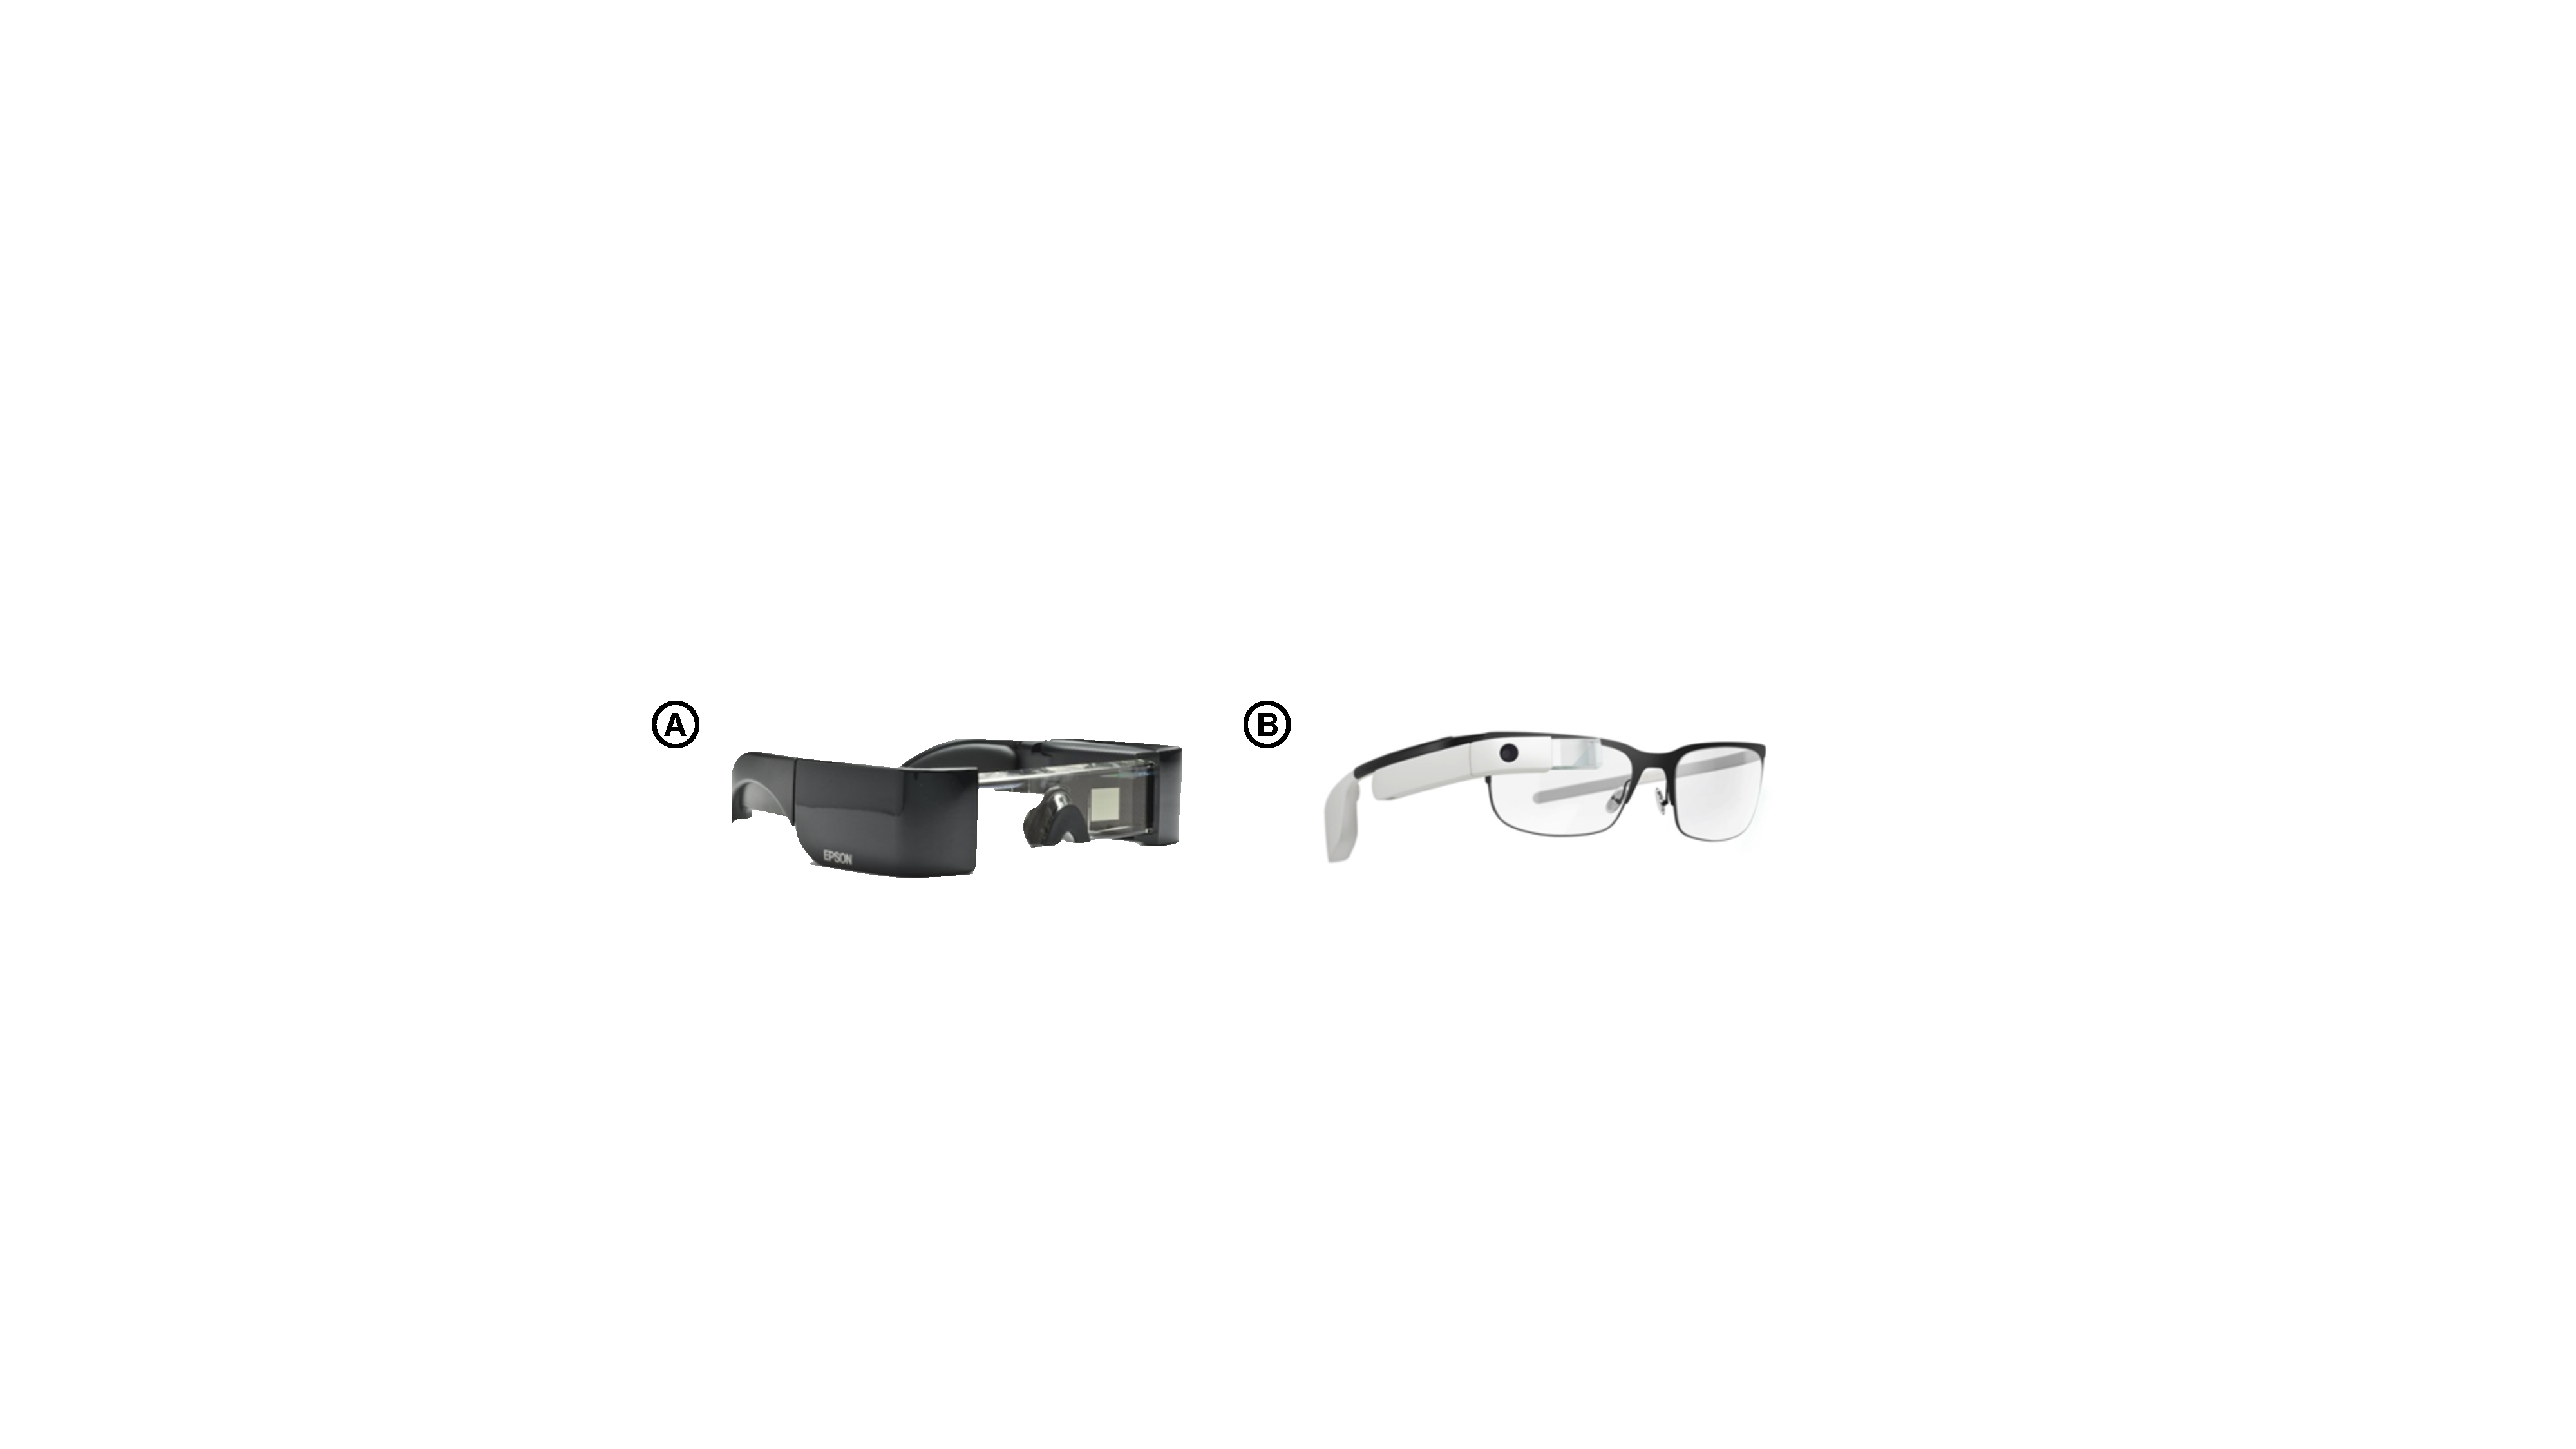
\includegraphics[width=1\columnwidth]{Glasses.pdf}
  \caption{(A) Epson Moverio, (B) Google Glass.}
  \label{fig:Glasses}
  \end{figure}

\subsection {Form Factor of Glasses}
We explored the form factors of smart glasses displays, and included both types in the study: 1) \emph{immersive}, which displays content spanning users' field of view (e.g. Epson Moverio), and 2) \emph{off-to-the-side}, with displays content in the corners of users' field of view (e.g. Google Glass)
The display of the Epson Moverio is located in front of the user's eyes with $960 \times 540$ resolution\cite{BT100}. And Google Glass locates its display above the user's right eye with $640 \times 360$ resolution\cite{GoogleGlass} (see Figure \ref{fig:Glasses}). 

  

  \begin{figure}[!h]
  \centering
  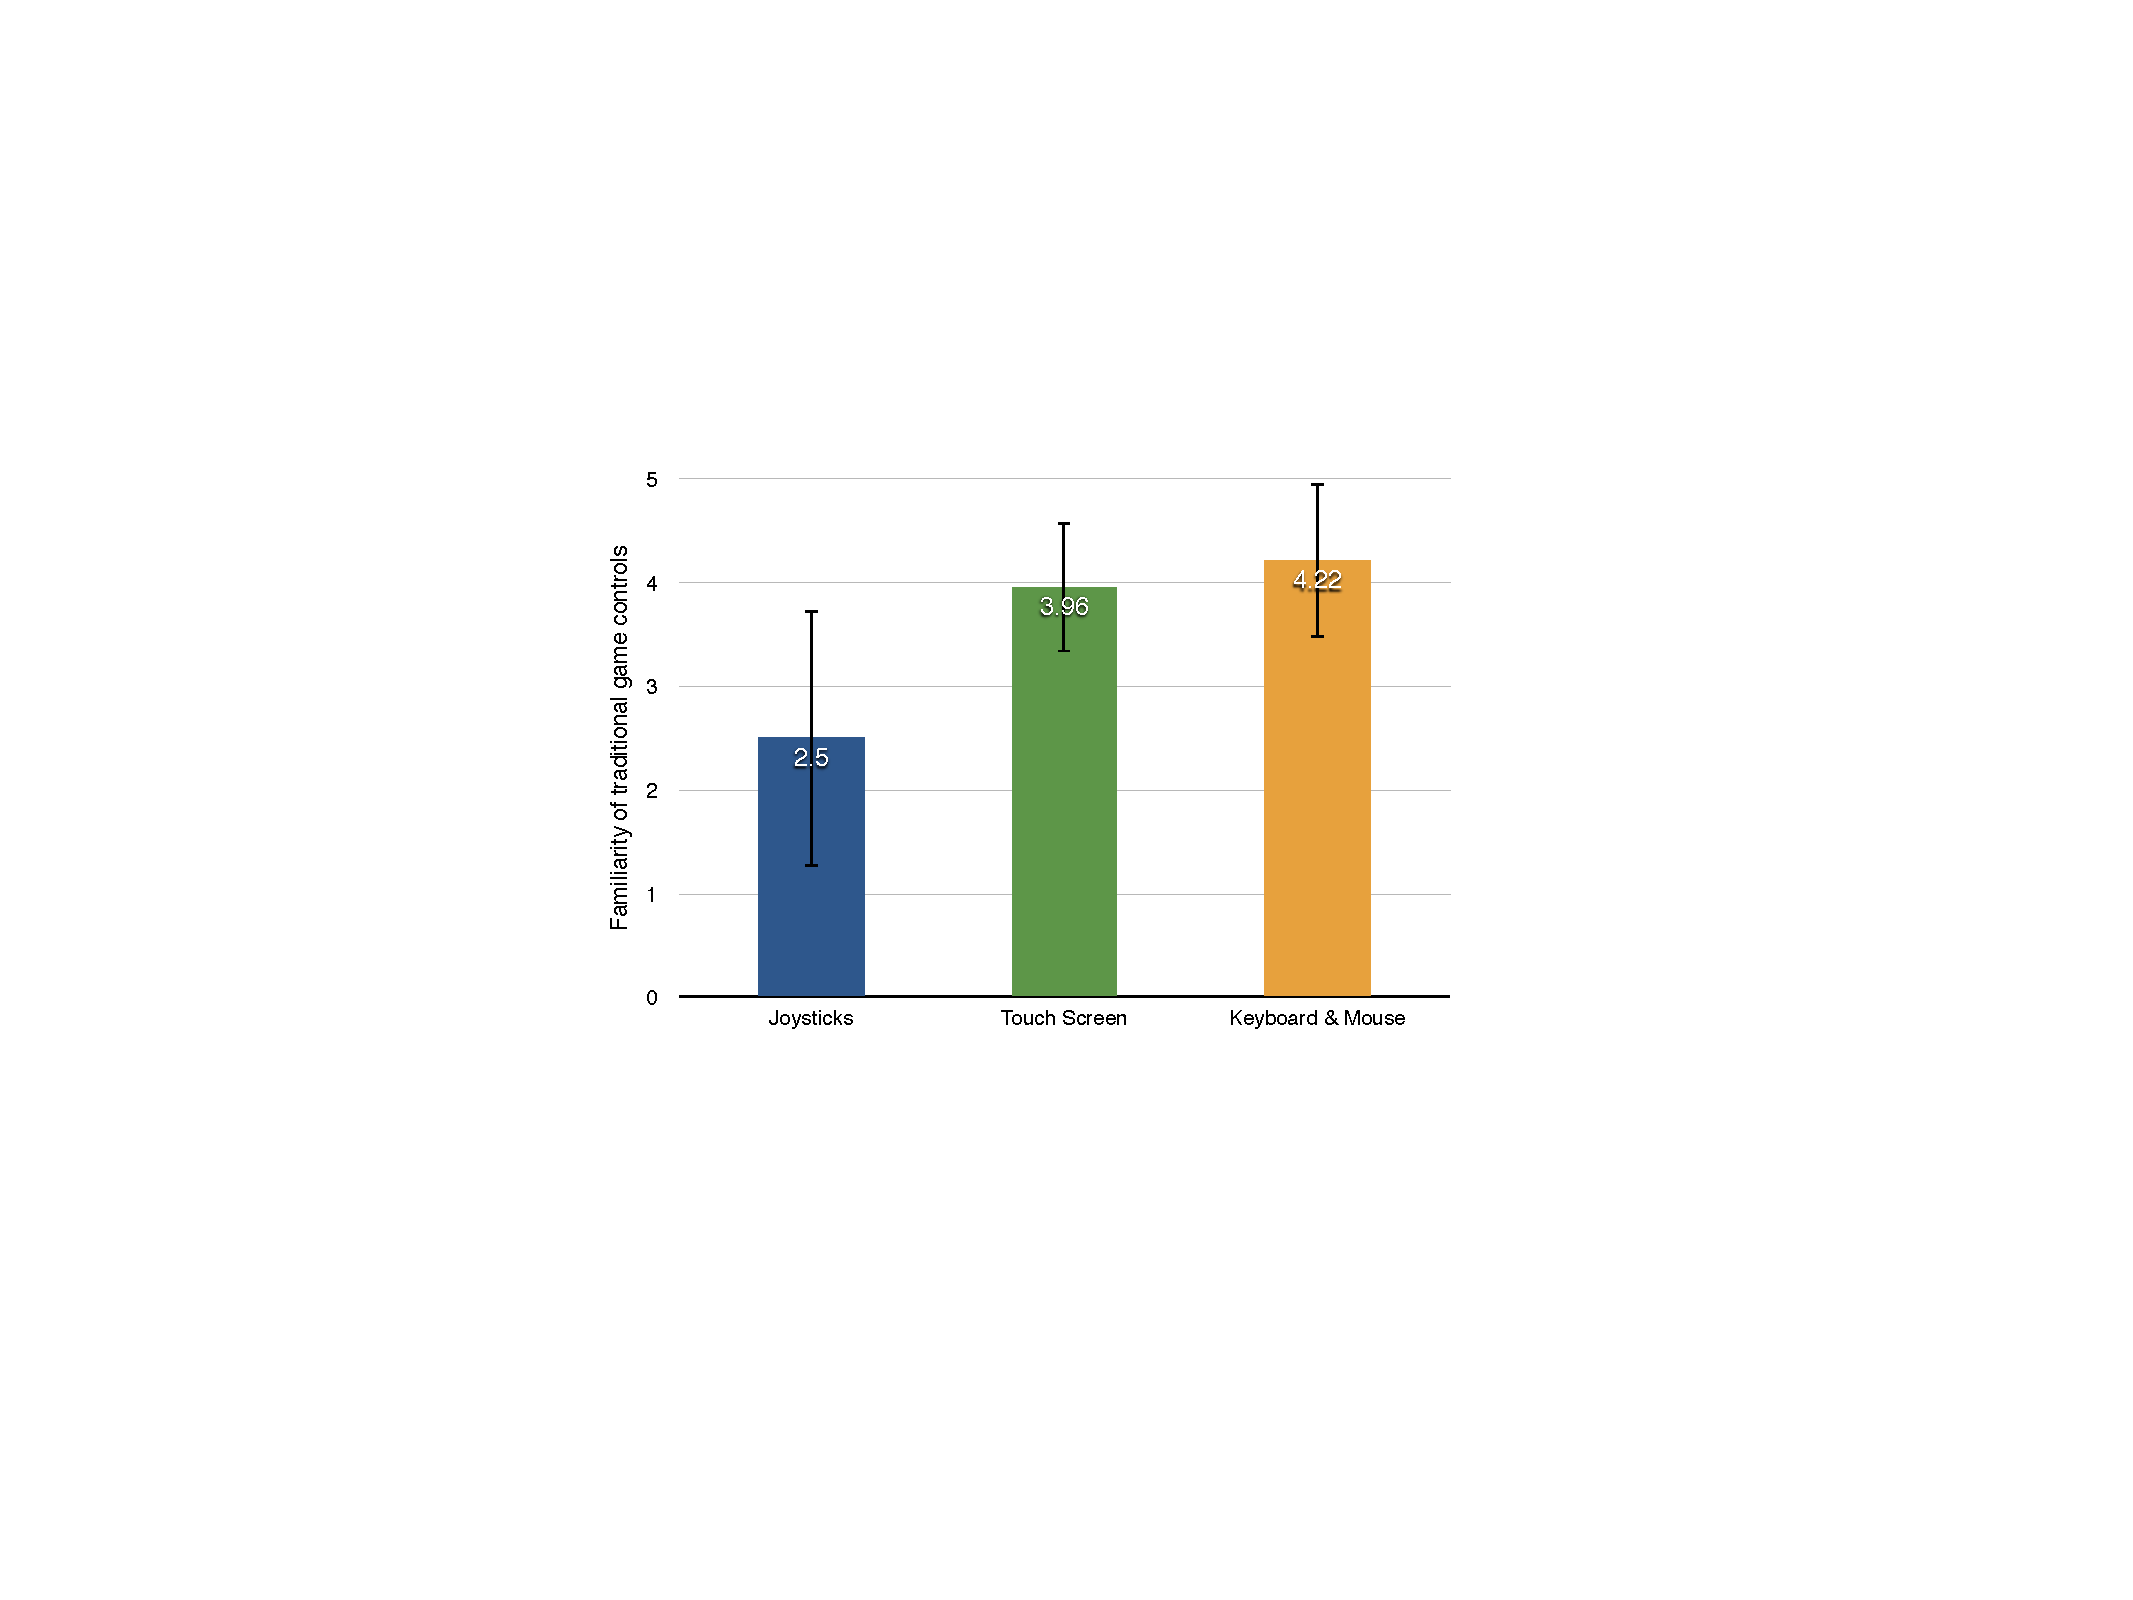
\includegraphics[width=1\columnwidth]{Familiarity.pdf}
  \caption{Users' game input familiarity.}
  \label{fig:figureFamiliarity}
  \end{figure}  

  \subsection {Participants}
  We recruited twenty-four participants with an equal male-female ratio for our study. Their average age was 23.2 (\textsl{sd} = 2.72). All participants are right-handed and none of them had past experience with smart glasses usage. About their gaming experience, according to our investigation, 14 users were daily game players, 9 were weekly players and 1 was a monthly player. Participants spent 1.36 hours (\textsl{sd} = 0.89) on average to play games one time. Moreover, 58\% of them indicated that their main gaming platforms were mobile phones, 38\% were on PCs, and only 4\% were on consoles. Another important factor of gaming experience is the familiarity of game controllers. The results showed that, compared with a game controller, most of them were more familiar with keyboards, mouses and touch screens (see Figure~\ref{fig:figureFamiliarity}).
  %\begin{figure}[!h]
  %\centering
  %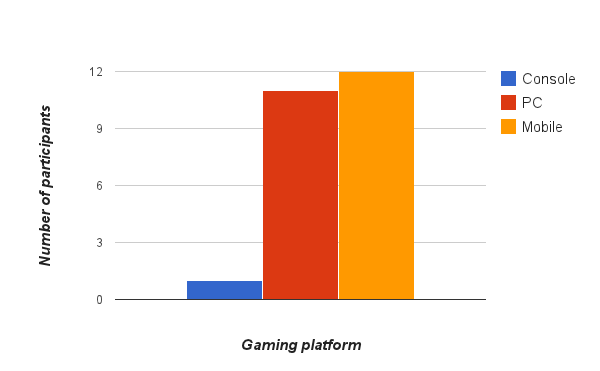
\includegraphics[width=0.9\columnwidth]{Platform}
  %\caption{With Caption Below, be sure to have a good resolution image
  %  (see item D within the preparation instructions).}
  %\label{fig:figurePlatform}
  %\end{figure} 
  %\begin{figure}[!h]
  %\centering
  %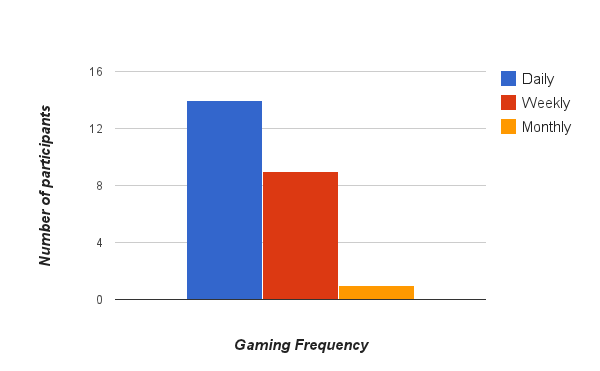
\includegraphics[width=0.9\columnwidth]{Frequency}
  %\caption{With Caption Below, be sure to have a good resolution image
  %  (see item D within the preparation instructions).}
  %\label{fig:figureFrequency}
  %\end{figure}
 

  \subsection {Environment}
  According to the previous works\cite{Wiliamson:2011:MMI:2070481.2070551,Williamson:2013:MEM:2522848.2522874,Montero:2010:YUS:1851600.1851647,Rico:2010:UGM:1753326.1753458}, the social acceptability of mobile-input was influenced by whether participants believed a bystander could interpret the intention of the input action. Therefore, to provide a game input set suited for a real-world environment, we chose a Starbucks cafe near our college. The visitor flow of the cafe, on average, was 72.5 persons per hour. In our investigation, participants indicated that the cafe was comparatively a public space with average 4.17 points (\textsl{sd}=0.65) on a 5-point Likert Scale for degree of field publicity (1 means very private, 5 means very public).    

  

    \subsection {Procedure}
    Participants wore two different glasses (Google Glass and Epson Moverio) and our software randomly presented 17 game tasks (Table \ref{tab:table1}) to participants. For each game task, participants performed a input action in 3 different interaction methods (\emph{handheld}, \emph{touch} and \emph{non-touch} interaction). The study was conducted using a counterbalanced measures design, alternating the glass's form and the interaction method. After each game input, participants were shown a 5-point Likert scale concerning subjective preference and conducted a short interview about input detail. With 24 participants, 17 game tasks, 2 glass forms and 3 interaction methods, a total of $24 \times 17 \times 2 \times 3$ = 2448 game input actions were made. 

    % these, 11 were discarded due to participant confusion. 

\section{Results}

Our results include game input taxonomies, user-defined game input set, user rating, subjective responses, and qualitative observations for each interaction method.

  \begin{table}
    \centering
    \begin{tabular}{|l|l|l|l|l|}
      \hline
      \tabhead{Method} &
      \multicolumn{1}{|p{0.13\columnwidth}|}{\centering\tabhead{Mean}} &
      \multicolumn{1}{|p{0.13\columnwidth}|}{\centering\tabhead{Std.}} &
      \multicolumn{1}{|p{0.13\columnwidth}|}{\centering\tabhead{L.Bound}} &
      \multicolumn{1}{|p{0.13\columnwidth}|}{\centering\tabhead{U.Bound}} \\
      \hline
      handheld & 3.68 & 0.79 & 3.63 & 3.74\\
      \hline
      touch & 3.77 & 0.81 & 3.72 & 3.83\\
      \hline
      non-touch & 3.81 & 0.90 & 3.75 & 3.87\\
      \hline

    

    \end{tabular}
    \caption{Summary of user preference of 3 different interaction methods, it provides mean value, standard deviation, and 95\% confidence interval for mean (Lower Bound and Upper Bound).}
    \label{tab:tablePreferenceInteractionMethod}
  \end{table}

  \subsection{Preference Between Interaction Methods}
  Table \ref{tab:tablePreferenceInteractionMethod} shows the average rating of 3 interaction methods. Three interaction types had a significant rating difference ($F_{0.05}$(2, 2445)=4.61, $p$ = .01). We found that the user rating preference for \emph{non-touch} was significantly higher than for \emph{handheld} ($p$ = .009). And we didn't find a significant difference between \emph{touch} and \emph{non-touch} ($p$ = .688).
  % , or on-body and phone interaction (P = .086). 
  In the interview conducted after the rating, we asked why users gave \emph{handheld} a lower preference score.
  The general reason was that users had to take out their controller, e g. phone, from their pocket. Users thought the handheld controller was not always-available and was not hands-free compared to the other interaction methods in this study. Considering the user preference, our report will focus on the results of \emph{touch} and \emph{non-touch} interaction without \emph{handheld} devices.



  \subsection{Behavior with Different Form Factor of Glasses}
  In our study, for each of the two glasses, there are 1224 game input pairs with the user, task and interaction method. We found 119 pairs of game input (9.72\% of all) were designed differently with distinct smart glasses forms. The influence of game input in each interaction method was 1.22\% for \emph{handheld}, 7.35\% for \emph{touch} and 20.59\% for \emph{non-touch}.

  While using \emph{non-touch} as interaction method, users who designed distinctive game input action mentioned that they were eager to use direct control and perfom a in-air gesture in front of the screen with the Epson Moverio. However, it is difficult to perform the same input with Google Glass because of the small screen size. On the other hand, users' reasons to define different input action with different glasses for \emph{touch} and \emph{handheld} interaction methods seem to be random as users were unable to motivate their choice to define a different input action.

  Although the form factor of smart glasses influenced the design of game inputs, there was almost no difference in the user preference ratings for user-defined game inputs between the 2 different glasses: ($F_{0.05}$(1, 2446)=.36, $p$=.549).


  \subsection{Classification of Game Inputs}
  %As noted in related work, ???????? . Ho however, no work has established a taxonomy of game control based on user behavior in public space to capture and describe the game design space.

   \begin{table}
    \centering
    \begin{tabular}{|c|l|c|}
      \hline
      \tabhead{\#} &
      \multicolumn{1}{|p{0.4\columnwidth}|}{\centering\tabhead{Task}} &
      \multicolumn{1}{|p{0.2\columnwidth}|}{\centering\tabhead{Kappa Value}} \\
      \hline
      1 & Select single from many& 0.863\\
      \hline
      2 & Vertical menu & 1.000\\
      \hline
      3 & Horizontal menu & 0.688\\
      \hline
      4 & Move left and right & 0.825\\
      \hline
      5 & Move in 4 directions & 1.000\\
      \hline
      6 & Switch 2 objects & 0.804\\
      \hline
      7 & Move object to position & 1.000\\
      \hline
      8 & Draw a path & 1.000\\
      \hline
      9 & Throw an object (in-2D) & 1.000\\
      \hline
      10 & Follow the beats & 0.697\\
      \hline
      11 & Rotate an object (Z-axis) & 0.867 \\
      \hline
      12 & Rotate an object (Y-axis) & 1.000\\
      \hline
      13 & Avatar jump & 0.867\\
      \hline
      14 & Avatar 3D move & 0.880\\
      \hline
      15 & Avatar attack & 1.000\\
      \hline
      16 & Avatar squat & 0.878\\
      \hline
      17 & Control 3D viewport  & 0.878\\
      \hline
      & \bf{Average} & \bf{0.897}\\
      \hline

    \end{tabular}
    \caption{Inter-rater reliability for each task.}
    \label{tab:kappa}
  \end{table}


  \subsubsection{Taxonomy of Game Input}
       
  As the authors, we manually classified the input actions along four dimensions: \emph{form}, \emph{binding}, \emph{nature}, and \emph{flow}. Within each dimension there are multiple categories as shown in Table \ref{tab:taxonomy}. To verify the objectivity (or inter-rater reliability), we invited an independent rater who performed the same categorization using 170 trials (10 trials were randomly selected for each task). The inter-rater reliability is shown in Table \ref{tab:kappa}. The lowest Kappa value, .688, is greater than .6, which is rated as \textsl{substantial} and thus is sufficient to establish the validity of the categorization. In addition, the average Kappa value is .897. A Kappa value of .8 and higher is considered \textsl{almost perfect}\cite{kappavalue}.



  

  The scope of the \emph{Form} dimension is applied separately to different interaction methods. There are 11 \emph{Form} categories with \emph{touch} input. 4 of them (\emph{palm}, \emph{back of hand}, \emph{forearm}, \emph{wrist}) are performed with both hands. 2 of them (\emph{leg}, \emph{face}) use a single hand to interact with other body parts. \emph{fingers} is a single hand input and it is merely an interaction between fingers, e.g. a pinch. And rest of them (\emph{ring}, \emph{watch}, \emph{glasses}, \emph{necklace}) are interactions with accessories. There are 4 form categories with the \emph{non-touch} interaction method. \emph{Finger} is a special case of \emph{hand}, but it is worth distinguishing because of its similarity to mouse actions and direct-touch.


  In the \emph{Nature} dimension, \emph{symbolic} inputs are visual depiction. For example, a user poses the v-sign in the air in order to select menu option 2, or forms his hand as a gun to throw an object. \emph{physical} inputs with the virtual object should be similar to the real world interaction with the physical object. \emph{metaphorical} inputs occur when a input acts on, with, or like something else. For instance, users trace a finger in a circle to simulate the ``object rotation'', or view the palm as a trackpad to perform gestures. As it should be, the input itself is usually not enough to reveal its metaphorical nature; the answer lies in the user's mental model which could be understood by the interview afterwards. Finally, \emph{abstract} inputs have no \emph{symbolic}, \emph{physical}, or \emph{metaphorical} connection to their game tasks. The mapping is arbitrary, which does not necessarily mean it is poor. Pinch-touching thumb and index finger to perform ``avatar jump'', for example, would be an abstract input.

The \emph{Binding} dimension is defined as the relationship between the input area and the smart glass's screen. \emph{direct} binding means the user performs the inputs in the screen region directly, such as using an in-air gesture right in front of the screen to drag or touch virtual objects. A game input binding is called a \emph{surface} binding if the user absolutely maps the screen onto another surface and performs the game inputs on it. Dragging a finger on the palm to move the object on the screen, for example, is a \emph{surface} binding input. For inputs categorized as \emph{independent} inputs it means that there is no binding between the screen and the input area. Thus the input can be performed in any position, like the ``pinch to jump''.

  A game input's \emph{Flow} is \emph{discrete} if the input is performed, delimited, recognized, and responded to as an event. An example is punching in the air to perform ``avatar attack''. \emph{Flow} is \emph{continuous} if ongoing recognition is required, such as during most of our participants' ``Control 3D viewport'' rotating the imaginary camera by hands. 

    \begin{table}
    \centering
    \begin{adjustwidth}{-0.5cm}{}
    \begin{tabular}{|l|l|l|}
      \hline
      \multicolumn{3}{|p{1.06\columnwidth}|}{\centering\tabhead{\textbf{Taxonomy of Game Inputs}}}\\
      \Xhline{4\arrayrulewidth}
        \textbf{\em{Form}} & \em{palm} & I.b. finger and palm. \\ \cline{2-3} 
        \textbf{\em{{\fontsize{0.3cm}{1em}\selectfont (touch)}}} & \em{fingers} & I.b. fingers.\\ \cline{2-3} 
             & \em{leg} & I.b. finger and leg.\\ \cline{2-3} 
             & \em{back of hand} & I.b. finger and back of hand.\\ \cline{2-3} 
             & \em{forearm} & I.b. finger and forearm.\\ \cline{2-3} 
             & \em{face} & I.b. finger and face.\\ \cline{2-3} 
             & \em{wrist} & I.b. finger and wrist.\\ \cline{2-3} 
             & \em{ring} & I.b. finger and ring. \\ \cline{2-3} 
             & \em{watch} & I.b. finger and watch.\\ \cline{2-3} 
             & \em{glasses} & I.b. finger and glasses.\\ \cline{2-3} 
             & \em{necklace} & I.b. finger and necklace.\\ 
       \Xhline{4\arrayrulewidth}
        \textbf{\em{Form}} & \em{finger} & Using finger to perform in-air gesture.\\ \cline{2-3} 
        \textbf{\em{{\fontsize{0.3cm}{1em}\selectfont (non-touch)}}}  & \em{hand} & Using hand to perform in-air gesture.\\ \cline{2-3} 
             & \em{head} & Using head to perform input.\\ \cline{2-3} 
             & \em{voice} & Using voice control.\\ 
      \Xhline{4\arrayrulewidth}
        \textbf{\em{Binding}} & \em{direct} & Directly control in front of screen. \\ \cline{2-3} 
             & \em{surface} & Absolute mapping screen to surface.\\ \cline{2-3} 
             & \em{independent} & No binding b. screen and input.\\
      \Xhline{4\arrayrulewidth}
        \textbf{\em{Nature}} & \em{symbolic} & Input visually depicts a symbol.\\ \cline{2-3} 
             & \em{physical} & Input acts physically on objects.\\ \cline{2-3} 
             & \em{metaphorical} & Input indicates a metaphor.\\ \cline{2-3} 
             & \em{abstract} & Input mapping is arbitrary.\\
      \Xhline{4\arrayrulewidth}
        \textbf{\em{Flow}} & \em{discrete} & Response occurs \em{after} the user acts.\\ \cline{2-3} 
             & \em{continuous} & Response occurs \em{before} the user acts.\\
      \hline
    \end{tabular}
    \caption{Taxonomy of game inputs based on 2448 input actions. The abbreviation ``I.b.'' means ``Interaction between''. The abbreviation ``b.'' means ``between''.}
    \label{tab:taxonomy}
    \end{adjustwidth}
  \end{table}
 

 \subsubsection{Taxonometric Breakdown of Input Actions in our Data}
We found that our taxonomy adequately describes even widely differing input actions made by our users. Figure \ref{fig:OnbodyTaxonomy} and \ref{fig:InAirTaxonomy} show for each dimension the percentage distribution between the categories. The \emph{Form} dimension for \emph{touch} input and the the \emph{Form} dimension for \emph{non-touch} input are both dominated with hand related input. And \emph{Form} dimension for \emph{touch} input is consisted of \emph{On-Body}(80.3\%) and \emph{Wearable}(19.7\%) interaction. We found that the forms of \emph{touch} inputs are more complicated than those of \emph{non-touch}. Nonetheless, the binding of \emph{touch} is more consistent. About 75\% of the inputs are independent of the screen. In addition, we were surprised that no user designed a \emph{direct} binding or \emph{physical} nature input with \emph{touch} input. And we found that for the \emph{Flow} dimension, the percentage distribution is similar for \emph{touch} and \emph{non-touch} interaction.

 \begin{figure}[!h]
  \centering
  \includegraphics[width=1.0\columnwidth]{OnbodyTaxonomy.pdf}
  \caption{Percentage of game inputs in each taxonomy dimension with \emph{touch} interaction. The  ``others'' on the form dimension is consisted of glasses (0.0164), necklace (0.0088), face (0.0075) and wrist (0.0025).}
  \label{fig:OnbodyTaxonomy}
  \end{figure} 

  \begin{figure}[!h]
  \centering
  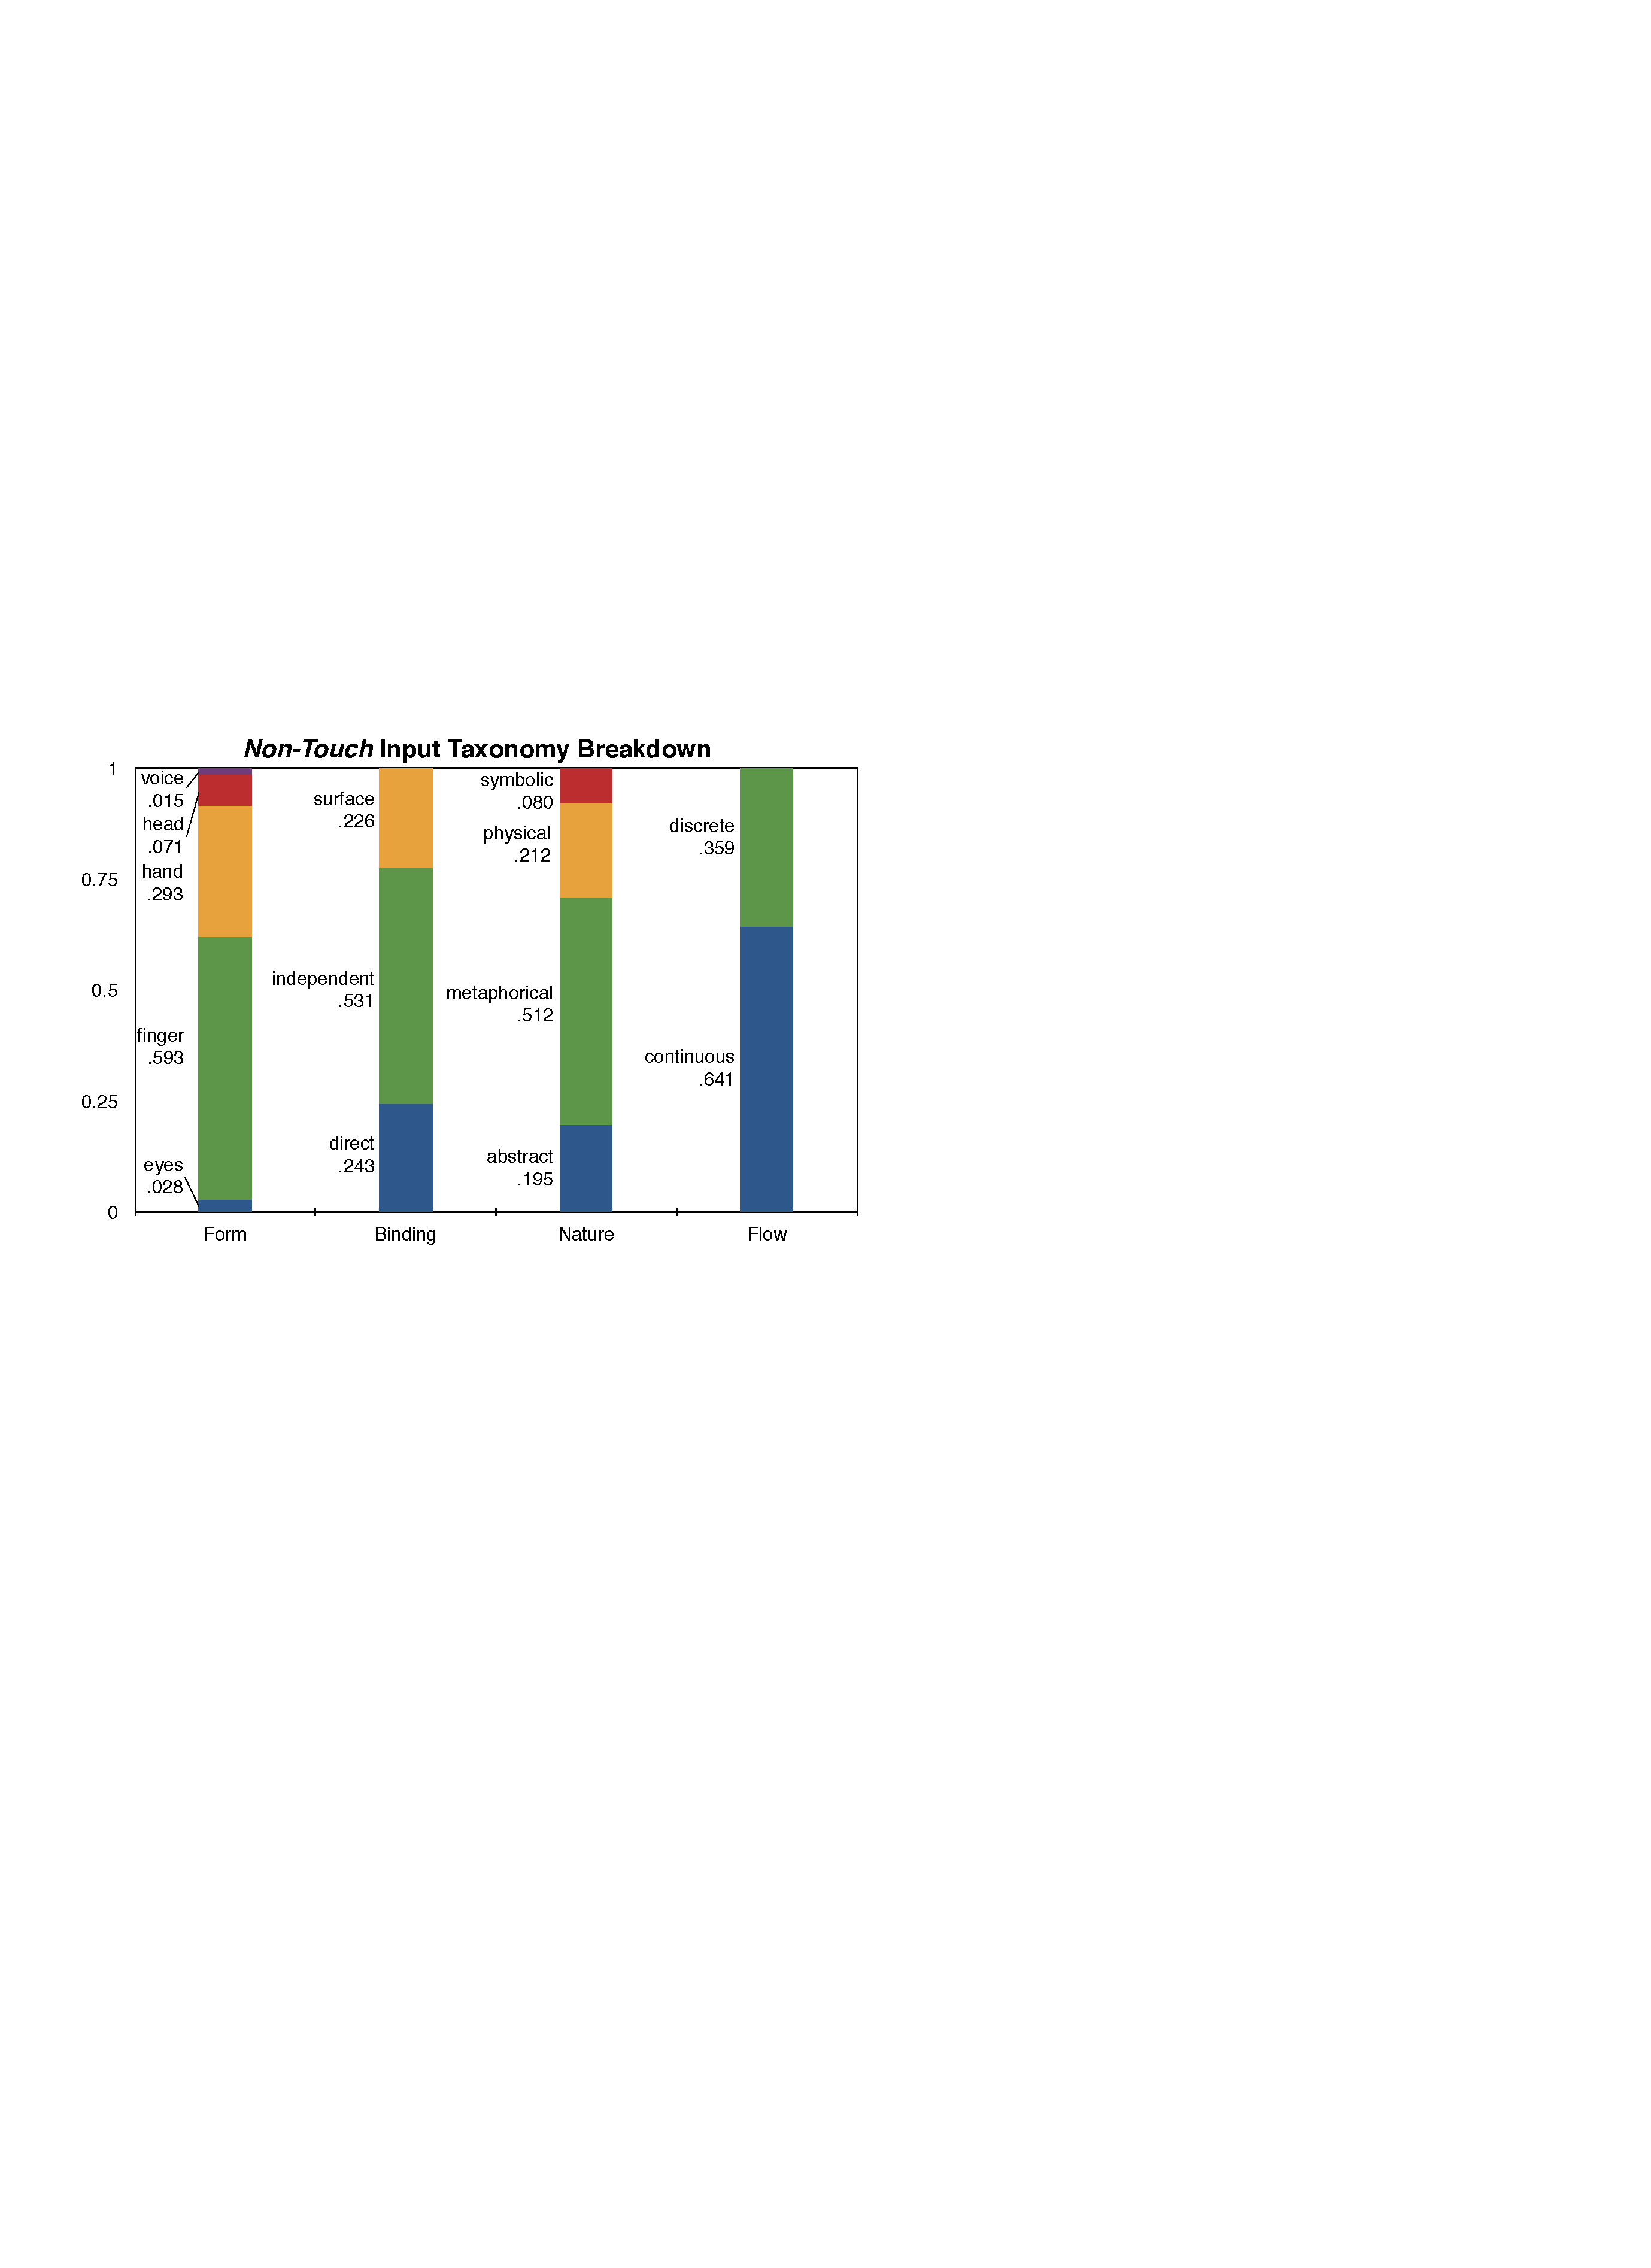
\includegraphics[width=1\columnwidth]{InAirTaxonomy.pdf}
  \caption{Percentage of game inputs in each taxonomy dimension with \emph{non-touch} interaction.}
  \label{fig:InAirTaxonomy}
  \end{figure} 

  \subsection{User-Defined Game Input Set}
  The goal of this work is to present a user-defined game input set for smart glasses used in a public environment. This section gives the process by which the set was created and properties of the set. Unlike the input sets for existing games on smart glasses, the set we have found is based on observed user behavior.

   \subsubsection{Agreement}
	All 24 participants have provided game input for each and every game task, smart glasses form and interaction method. For each game task we made groups of identical actions used by participants. Group size was then used to compute an \emph{Agreement Score} that reflects the consensus among participants regarding the action used for a certain game task. A task with a .31 agreement score means that, two randomly picked participants will have a 31\% chance to perform an identical input action for this task. The definition and formula of the agreement score can be found in previous work. \cite{Wobbrock:2005:MGS:1056808.1057043}.
   \begin{equation}
   A = \frac{\displaystyle{\sum_{t\epsilon T }} \sum_{P_i \subseteq P_t } \left(\frac{\lvert{P_i}\rvert}{\lvert{P_t}\rvert}\right) ^ 2}{\displaystyle{\lvert{T}\rvert}}
   \end{equation}
  
   In eq. 1, $t$ is a task in the set of all tasks $T$, $P_{t}$ is the set of proposed input actions for task $t$, and $P_i$ is a subset of identical input actions from $P_{t}$. The range for $A$ is $\left[\lvert{P_t}\rvert ^{-1}, 1\right]$. As an example, consider the agreement for \emph{draw a path} with \emph{touch} input, it had four groups of identical input actions with group sizes 34, 4, 5 and 5. we compute

   \begin{equation}
   A_{touch-path} = \left(\frac{34}{48}\right) ^ 2  + \left(\frac{4}{48}\right) ^ 2 + \left(\frac{5}{48}\right) ^ 2 + \left(\frac{5}{48}\right) ^ 2 = 0.53
   \end{equation}

The participant agreement for our study is pictured in Figure \ref{fig:Agreement}. The overall agreement for \emph{touch} and \emph{non-touch} inputs were $A_{touch}$=0.25 and $A_{non-touch}$=0.27, respectively. When comparing the agreement of \emph{touch} and \emph{non-touch} inputs, we clearly see that their patterns are extremely similar. The average difference of agreement between these two interaction methods was .056. This implies that the agreement score was influenced more by the game tasks than by the interaction methods.


 \begin{figure}[!h]
  \centering
  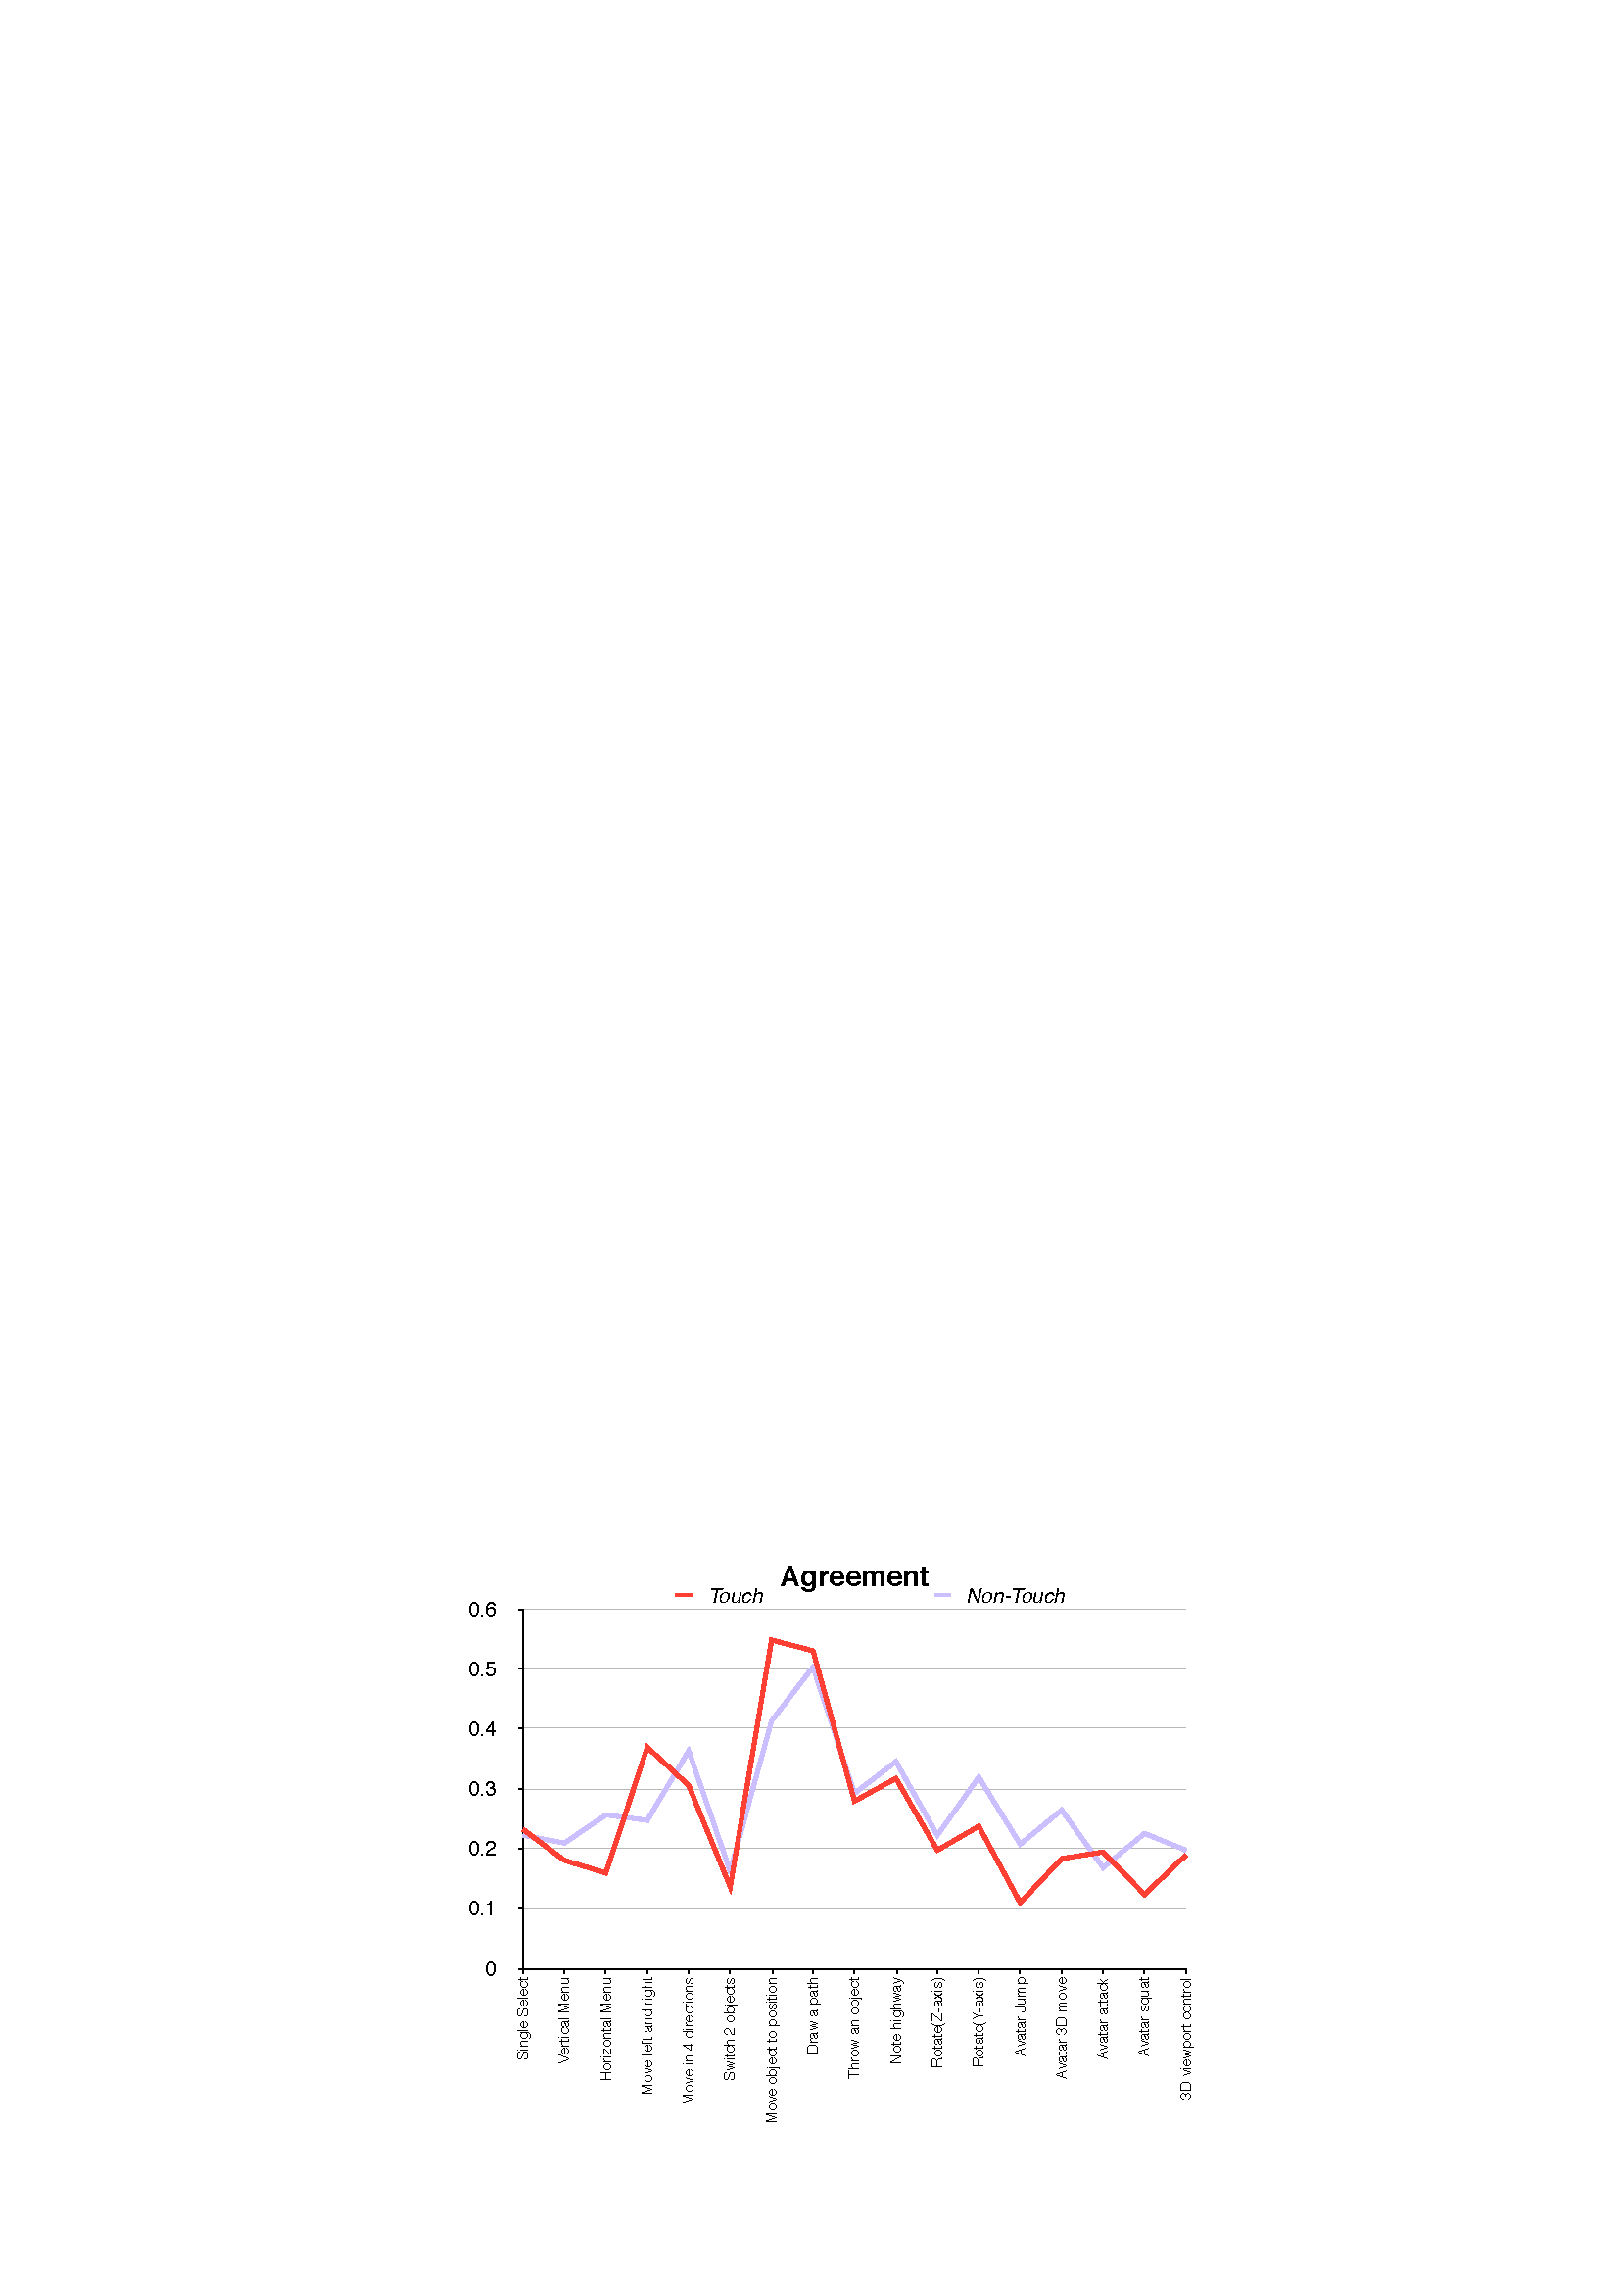
\includegraphics[width=1\columnwidth]{Agreement.pdf}

  \caption{Agreement for each game task. The tasks are listed in the same order as they appear in Table \ref{tab:table1}.}
  \label{fig:Agreement}
  \end{figure} 

   %\subsubsection{Conflict and Coverage}

   %Howerver, where the same control action was used to perform different game tasks, a conflict occurred if the game consists the tasks at same time. In our case ,we found that ``Move in 4 Directions'',``Avatar 3D Move'' and ``Viewport Controls'' are assigned with same control action with on-body input(Fig?.?). According to the property of our top 90 casual games, the average task count for these game is 2.56 (std=1.07). In another word, there are about 1 to 4 game tasks in each game title. There is a low chance to perform these three game controls at same game and same time. To make our game control set reflects more consistent with user behavior, we decide to remain it conflict. 


   \subsubsection{Properties of the User-defined Game Input Set}
   The user-defined game input set was developed by taking the largest groups with identical input actions for each game task and assigning those actions to the game tasks. 
   The resulting user-defined game input set includes inputs for both the \emph{touch} and the \emph{non-touch} interaction class with agreement scores of 41.32\% and 40.07\% respectively. Our user defined set is useful, therefore, not just for what it contains, but also for what it omits.

      All the inputs in our final \emph{touch} input set are finger based (see Figure \ref{fig:OnBodyInputSet}). Most of them use a single finger tip to perform gestures on different surfaces. The most preferable surface for \emph{touch} input is the hand palm. This way, the hand palm acts as a trackpad or a proxy touch-screen. The other touch inputs are finger interactions with single hand. More specifically, participants used their thumb to interact with their index finger or the ring on the finger.

   For \emph{non-touch} input set (see Figure \ref{fig:InAirSet}), even though we informed users beforehand that they were not limited to using their hands when providing game input, the results show that users still preferred to use hand input over voice control, eye gestures and head tilting. Additionally, users would make use of direct-control if they had to perform precise tasks, such as selecting an object from many or moving an object to a specific position. On the other hand, for tasks with lower precision requirements, such as selecting a single option from 4 or making an avatar jump, users would prefer using an indirect-control. For examples: the user taps 4 different areas in front of their chest or the user raises his hands slightly.


 

   \subsubsection{Taxonometric Breakdown of User-Defined Game Inputs}
   As expected, the taxonometric breakdown of the final user-defined game input set (Figure \ref{fig:OnBodyInputSet} and \ref{fig:InAirSet}) is similar to the proportions of all control actions proposed (Figure \ref{fig:OnbodyTaxonomy} and \ref{fig:InAirTaxonomy}). Across all taxonomy categories, the average difference between these two sets was only 4.7\%, (\emph{touch} input 6.31\% and \emph{non-touch} input 3.09\%, respectively).

  \subsection{Mental Model Observations}
    \subsubsection{Social Acceptance and Input Area}
    To our surprise, approximately 63\% of the in-air gestures were not performed in front of the face (See Figure \ref{fig:figureInAirPorpotion}.2). This behavior conflicts with the current ``Google Glass'' design. There were 7 participants who performed most gestures in front of their face. They indicated that input in front of the face was more precise and intuitive. At the same time, the other 17 participants preferred to perform in-air gestures in front of or below their chest. Among them, there were 3 participants who didn't perform a single in-air gesture in front of their face. These users indicated that moving a finger in front of their face was weird and not socially acceptable. They also noted that there was a hand fatigue problem if they had to lift their hand in front of their face all the time, so they thought that it was not suitable for gaming.

    \subsubsection{Bias by Existing Game Input}
    Although we were careful not to show elements from traditional game platforms like PCs, consoles and mobile games, participants still often reasoned based on their previous gaming experience. For example, some input actions were performed as if using a touch-screen in front of their face (see Figure \ref{fig:InAirSet}\{A,F,G\}). Some actions were like using an imaginary trackpad on an in-air surface or on the hand palm(see Figure \ref{fig:OnBodyInputSet}\{B,D,E,H,I,K,N,Q\} and Figure \ref{fig:InAirSet}\{H,I\}). Even with simple shapes and basic characters, it was clear how deeply rooted the previous gaming experience is. Some quotes reveal this: ``So I just click a button like on a game controller'', ``Can I just imagine there is a trackpad on my palm?'' and ``It's an imaginary touch-screen.''

\subsubsection{Identical Gestures on Different Surfaces}
 In our study, we found several identical gestures performed by our users on different surfaces. Take the task ``Move in 4 directions'' for example, although 57\% of the gestures were performed by moving a finger on the palm with \emph{touch} inputs(Figure \ref{fig:OnBodyInputSet}.E). The rest of the gestures were mostly using identical gestures (moving a finger), but then on the different surfaces such as the back of the hand, the leg, the forearm and on the even face. The same phenomenon could also be observed when comparing the game input of the user-defined input set with \emph{touch} and \emph{non-touch} inputs for the tasks ``Move left and right'', ``Move in 4 directions'', ``Draw a Path'', ``Throw an Object''. Participants used the hand palm or an imaginary in-air surface. 
 (See Figure \ref{fig:OnBodyInputSet} and Figure \ref{fig:InAirSet} \{D,E,H,I\}). In these cases, the surface did not influence the meaning of the gestures. We have asked users why they chose the palm as their input area. The general response was that it required the least physical movement, such as ``I chose the left palm to perform a gesture on because it is near to my right index finger''. 

  \section{Discussion}
    %\subsubsection{Users' and Designers' Gestures}

    \subsubsection{Implications for Touch Input Technology}
    Our results showed that the hand palm was the most favorite area for users to perform \emph{touch} inputs on. Half of the game inputs with \emph{touch} input used a finger to perform a gesture on the palm (See Figure \ref{fig:figureOnBodyPorpotion}). According to the mental model mentioned above, users utilized the metaphor of a trackpad and a touch-screen on the palm in several cases. Gesture-recognition on the hand palm might be a applicable for these input actions.

    %From another point of view, since all these inputs were performed with fingers of users' dominant hand. If possible, we would suggested that the sensing area should be located around the index finger of the dominant hand instead of on specific body parts, such as a palm or leg. This would enable the user to use any surface for touch input. 

   \begin{figure}[!h]
    \centering
    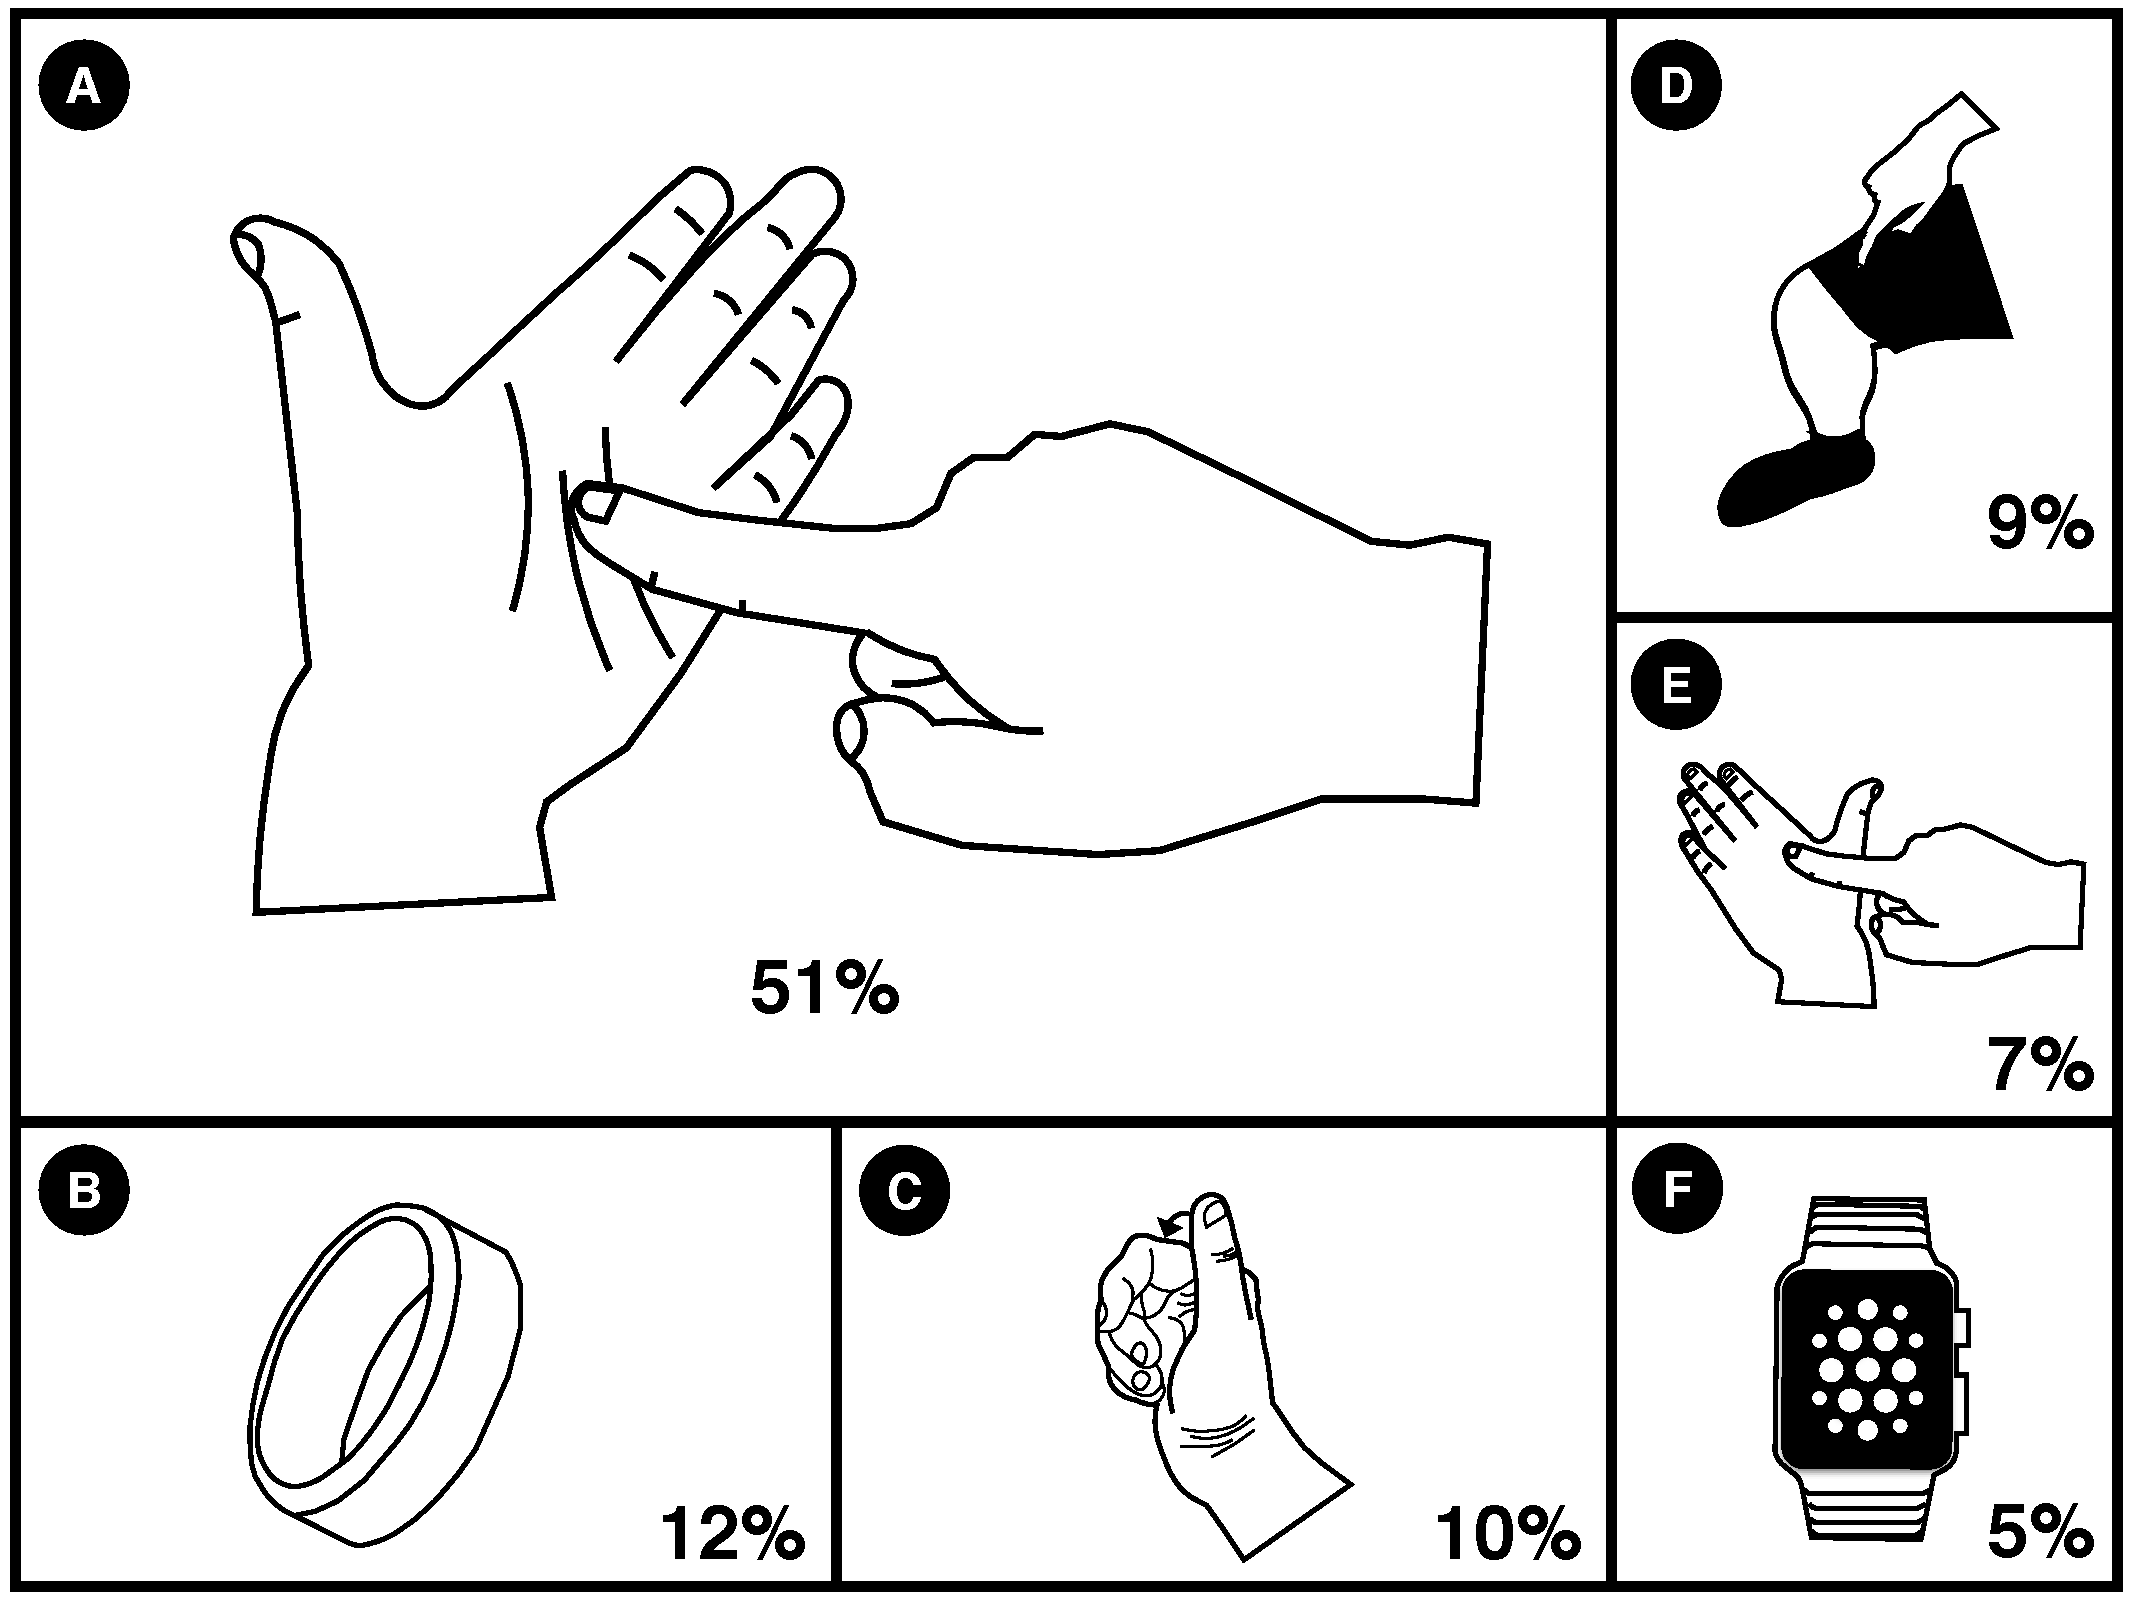
\includegraphics[width=0.9\columnwidth]{OnBodyForms.pdf}
    \caption{The top 6 \emph{touch} input forms. Percentage indicates the portion of \emph{touch} input actions. (A)Interaction between finger and palm. (B)Interaction between finger and ring. (C)Interaction between fingers. (D)Interaction between finger and leg. (E)Interaction between finger and back of hand. (F)Interaction between finger and watch.}
    \label{fig:figureOnBodyPorpotion}
    \end{figure}   


  \begin{figure*}
  \centering
  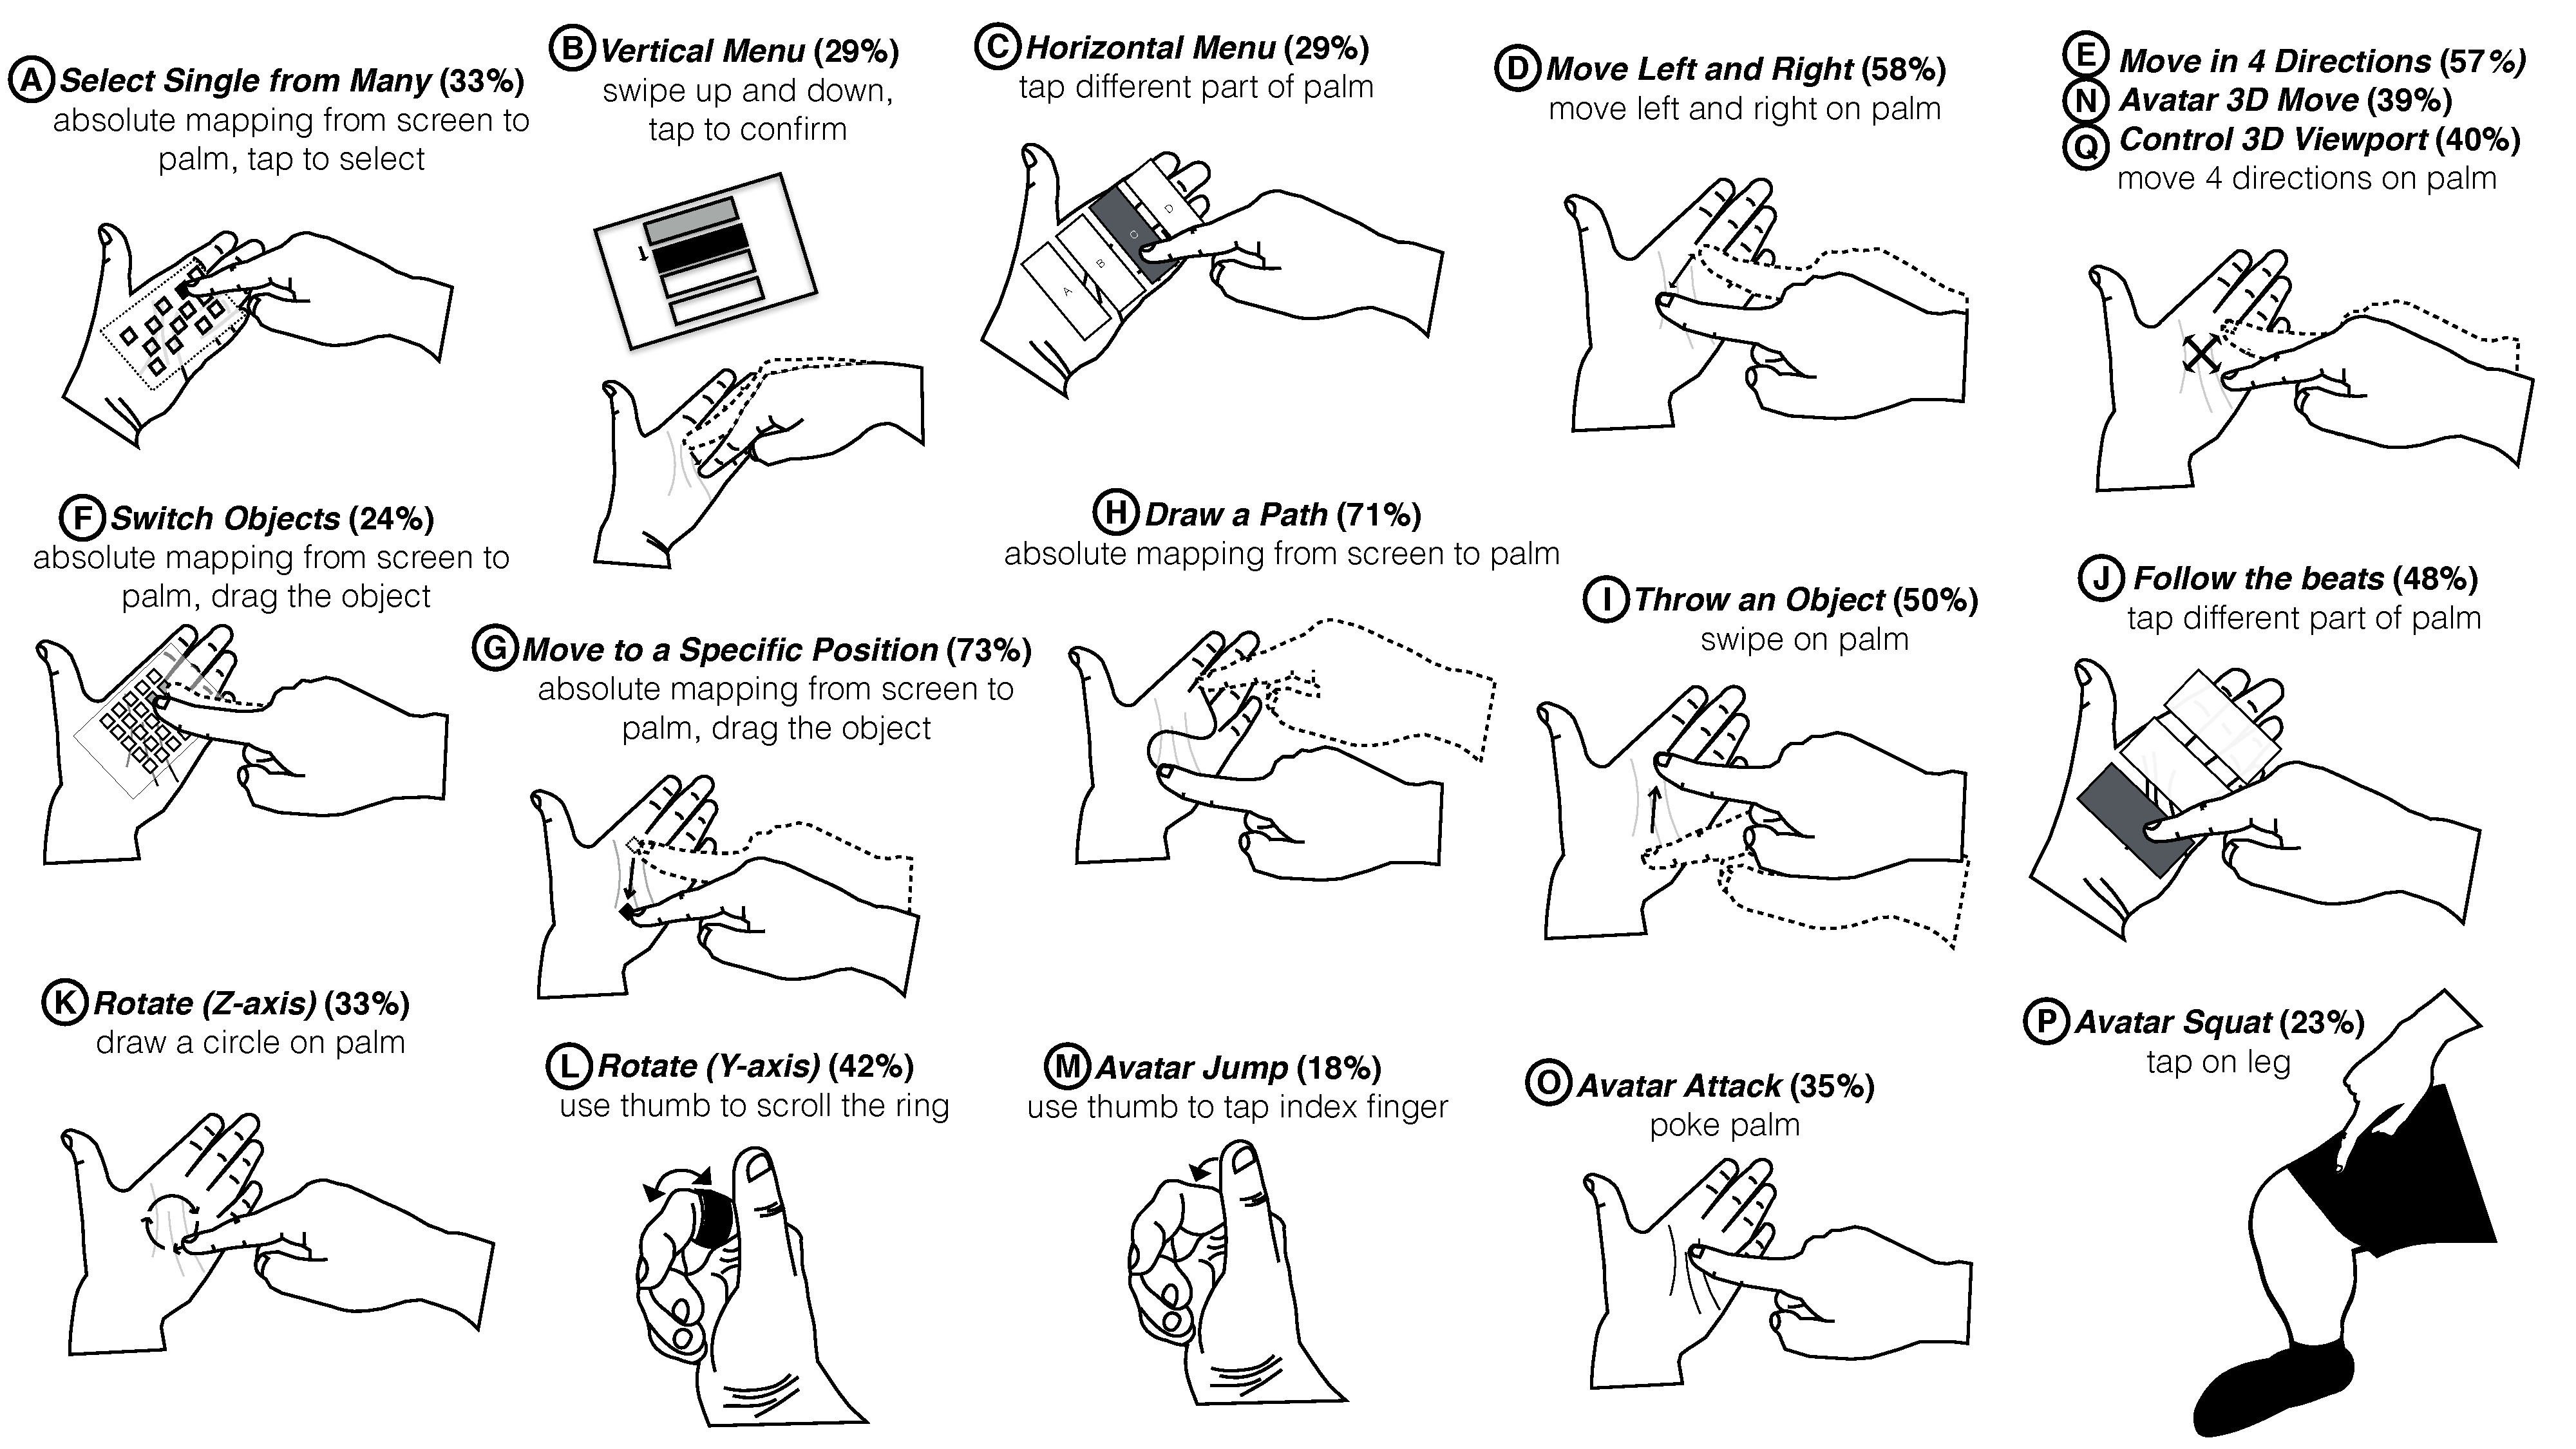
\includegraphics[width=1\textwidth]{OnBodyInputSet.pdf}
  \caption{The user-defined game input set with \emph{touch} inputs. The percentages indicate the portion of users who performed the pictured input action for the game task. Note that, there are 3 tasks (``Move in 4 directions'', ``Avatar 3D Move'', and ``Control 3D viewport'') have been assigned with an identical input action.}
  \label{fig:OnBodyInputSet}
  \end{figure*}

  \begin{figure*}
  \centering
  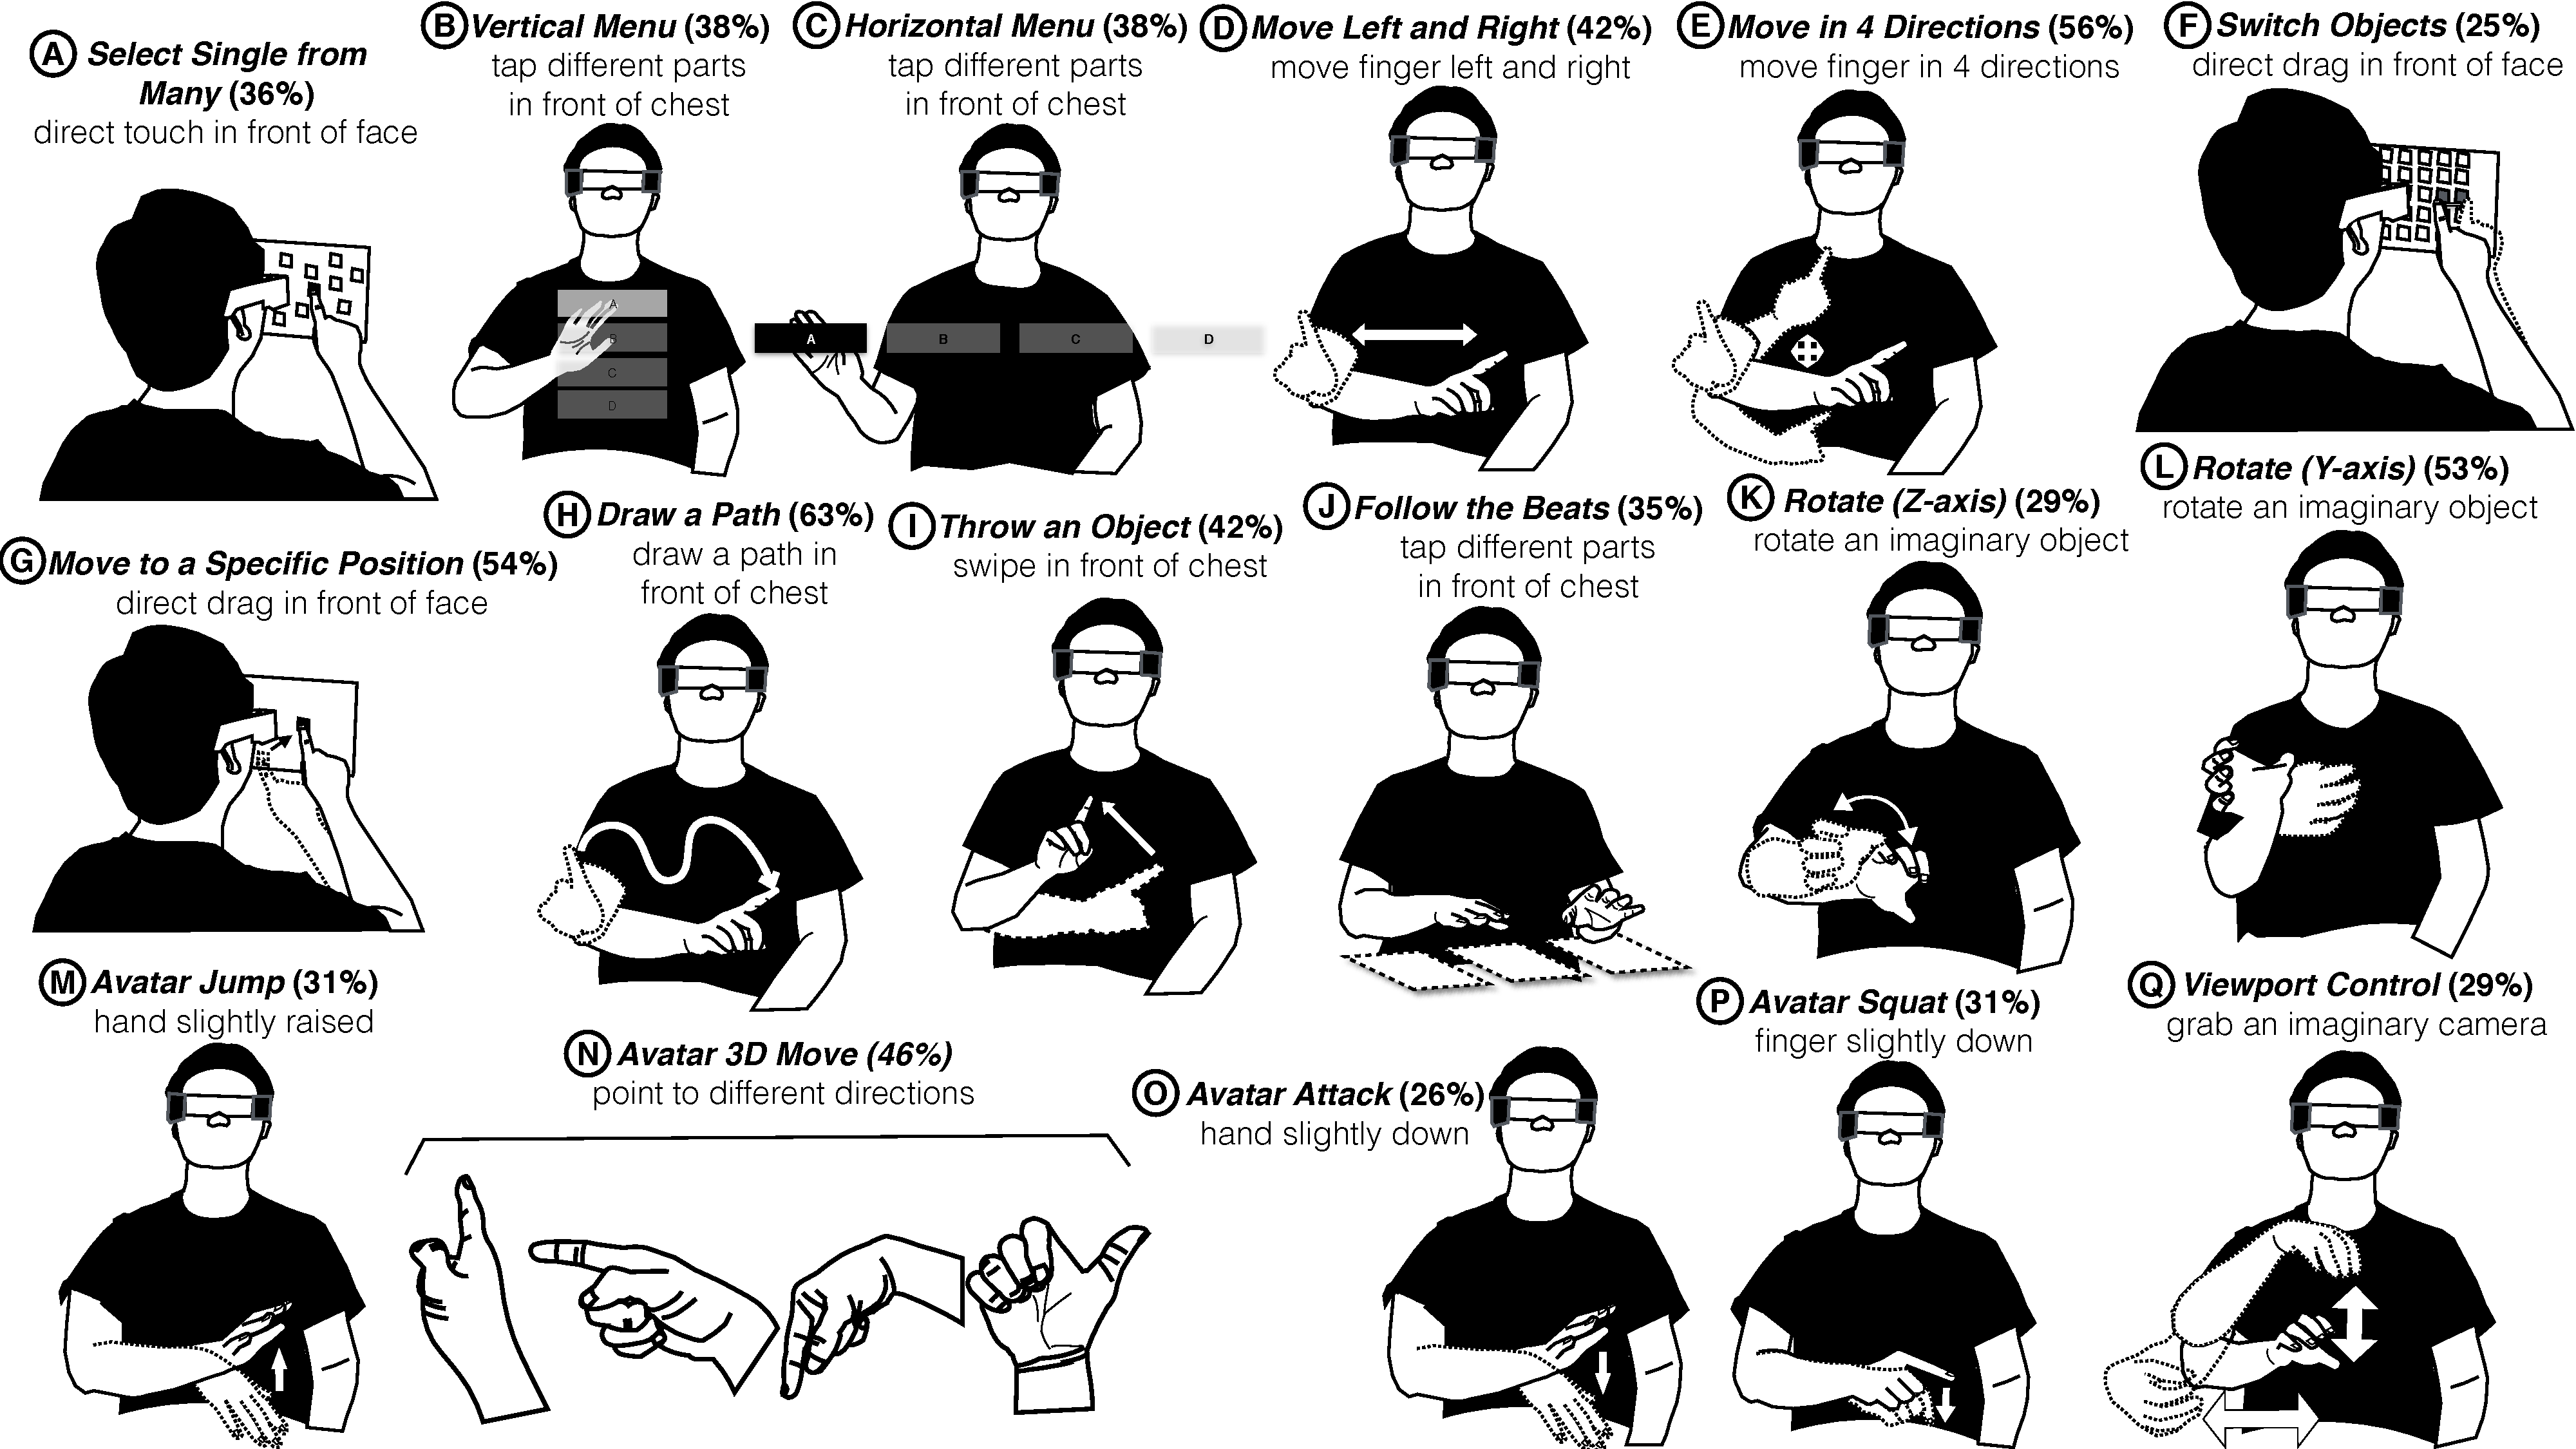
\includegraphics[width=1\textwidth]{InAirSet.pdf}
  \caption{The user-defined game input set with \emph{non-touch} interaction, The percentages indicate the portion of users who performed the pictured input action for the game task.}
  \label{fig:InAirSet}
  \end{figure*}

    \subsubsection{Implications for Non-Touch Interaction Technology}
    For \emph{non-touch} interaction methods, our taxonomy shows that performing in-air gestures with fingers and hands are still the dominant forms for smart glass gaming (Figure \ref{fig:figureInAirPorpotion}.1\{A,B\}). There was only a small number of participants that used head-gestures, eye-gestures or voice controls, 7\%, 3\% and 1\% respectively.
    Before our study, both Google Glass and Mime\cite{GoogleGlass, Colaco:2013:MCL:2501988.2502042} supplied their own in-air gesture sets to increase the diversity of their input. However, our results show that 63\% of the in-air gestures are not performed in front of the user's face in the public space due to the social acceptance issues and physical tiring problems mentioned before (see Figure \ref{fig:figureInAirPorpotion}.2). Therefore, if the developers of head-worn devices want to implement in-air gestures for input, they will need to have the capability to sense gestures in a wide range of areas near the user other than only right in front of the face. Take CV-based sensing technologies for example, instead of a regular lens, we could use a wide-angle lens or fish-eye lens to implement a system to cater to the user's preference.   
  \begin{figure}[!h]
  \centering
  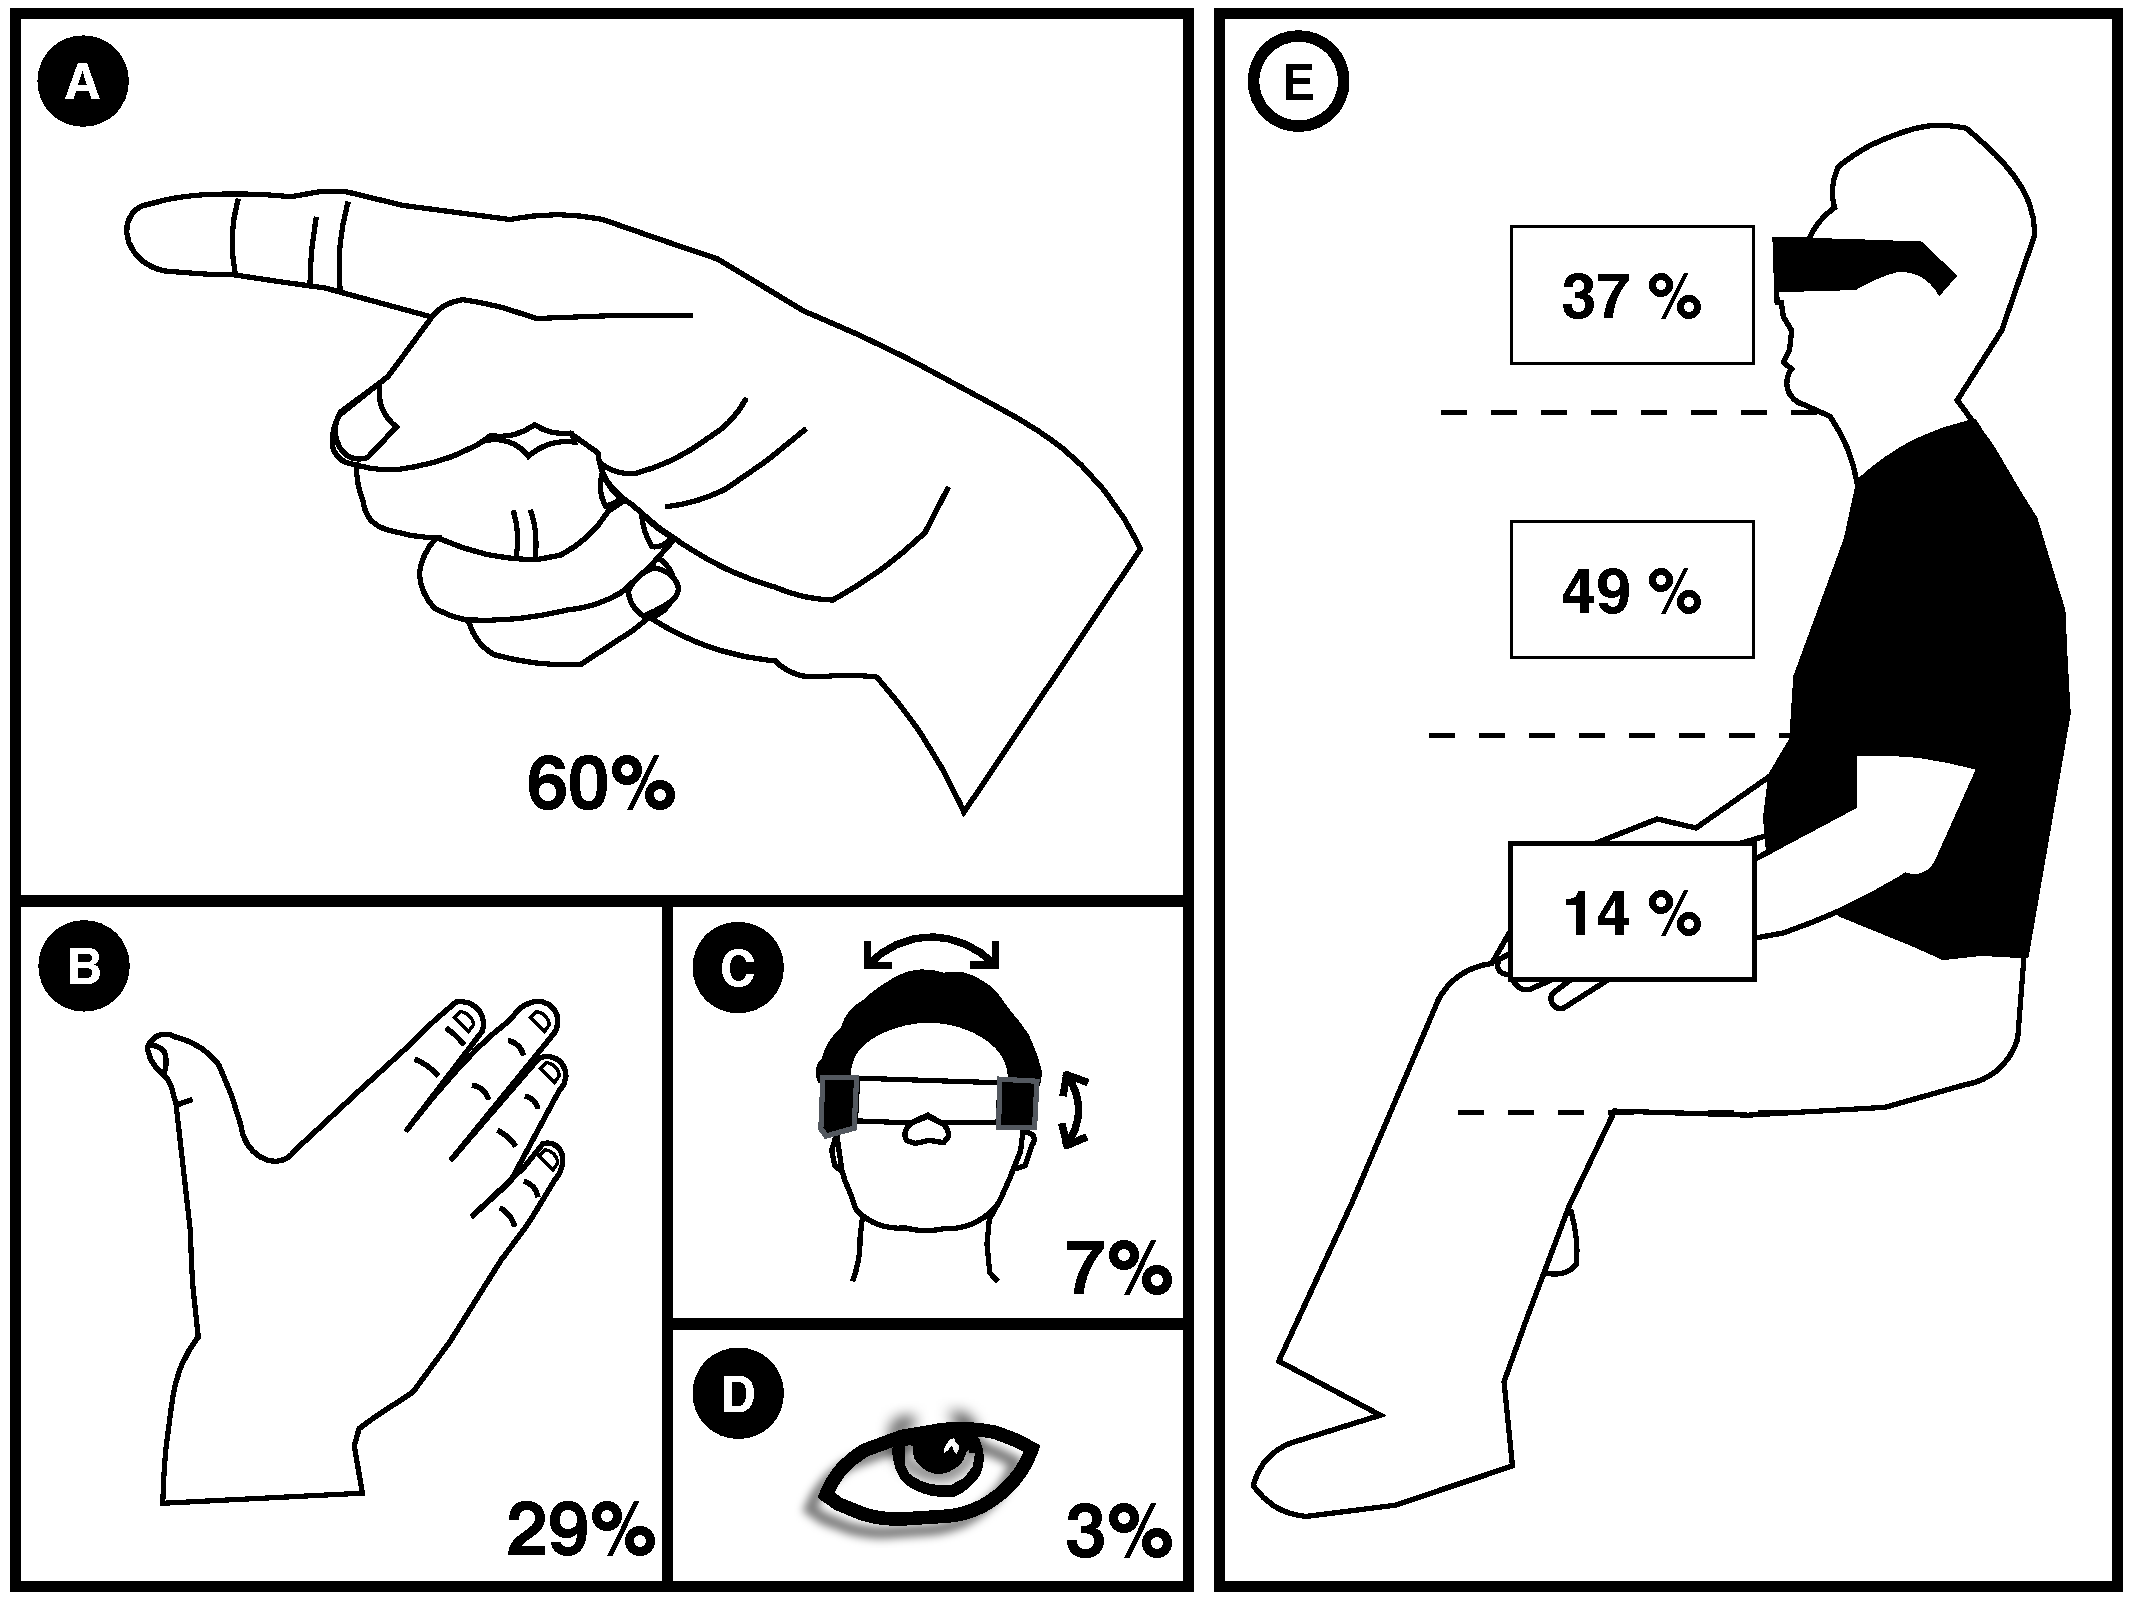
\includegraphics[width=0.9\columnwidth]{InAirControlArea.pdf}
  \caption{1. The top 4 \emph{non-touch} interaction forms. Percentages indicate the portion of \emph{non-touch} game inputs that consisted of the pictured input. (A) Using a finger to perform an in-air gesture. (B) Using the full hand to perform an in-air gesture. (C) Using head-tilting or rotating to perform game input. (D) Using eye-gestures to perform game input. 2. The distribution of the in-air gesture input area. Half of the in-air gestures (49\%) were performed in front of the chest, 14\% in front of or below the belly, and only 37\% of the gestures were performed in front of the face.}
  \label{fig:figureInAirPorpotion}
  \end{figure}







  \subsubsection{Implications for Game Design}
  According to the agreement scores we found that, no matter if using \emph{touch} interaction or \emph{non-touch} input, the average agreement between users was only .26, and the highest agreement was just about .55 (see Figure \ref{fig:Agreement}). In this case, guessing the game inputs would become a frustrating experience for players. It indicated that game developers should design the visual guide carefully to lead users performimg the input action, or show a instruction to explain the input methods.




  %\subsubsection{Implications for User Interfaces}
  \subsubsection{Limitation and Next Steps}

  In our work, we showed every single game task independently to the participants. Participants designed inputs for these tasks without an overview of all tasks. The input actions in our resulting set might have conflicted with each other if we wanted to perform two or three inputs simultaneously. For example, with \emph{touch} input, users would maybe feel uncomfortable to ``Move in 4 directions'' and perform ``Avatar attack'' at the same time (see Figure \ref{fig:OnBodyInputSet}\{E,O\}). In the future work, we will try to show users a combination of multiple tasks and to understand more about the difference of the users' behavior under this circumstance.

  As we know, there are many different places known as public space, and users may behave differently in each specific place. Furthermore, in our study, we did not ask users to define any input actions to interact with tangible objects in public space, such as, tables or chairs in the cafe shop. We only made participants experience two types of smart glasses. Therefore, our user-defined game input set might not be suitable to be applied to games on other types of head-worn devices. Moreover, our participants were all literate Taiwanese adults; undoubtedly, children, elders, participants form other cultures, or uneducated participants would behave differently. That is to say, these issues are worthy of investigation, but exceed the range of our current work.

  An important next step is to validate our user-defined game input set with a wearable system, which can sense all \emph{touch} and \emph{non-touch} input actions listed in our set.   
    %Glass Forms 只有兩種
    %Culture問題?
    %Interaction with 桌椅?


\section{Conclusion}

This paper explored user-defined game input for smart glasses beyond the capabilities of current sensors, and focused on gaming interaction in public settings. We conducted a user-defined input study with 24 participants, each performing 17 common game control tasks using \emph{handheld}, \emph{touch} and \emph{non-touch} interaction methods with two form factors of smart glasses in a public cafe, which lead to a total of 2448 game inputs. Our results indicate that participants significantly preferred \emph{non-touch} interactions over \emph{handheld} interactions (3.81 vs 3.68, $p$ \textless 0.01). And the most frequently used body surface was the palm (51\%). Also, participants preferred using in-air gestures in front of the torso over gestures in front of the face(63\% vs 37\%) due to concerns with social acceptance and the hand fatigue issue. Furthermore, we indicated the mismatch between participants' preferred input methods and those supported by current smart glasses.

The contribution of this paper are as follows: (1) the first quantitative and qualitative characterization of user-defined input for games on smart glasses, including a taxonomy, (2) set of user-defined input for common game tasks for non-handheld input methods, which is reflective of user behavior. (3) insight into users' mental models when playing smart glasses games in a public space, and an understanding of implications for mobile input technology and user interface design.

This work represents a necessary step in bringing glassses gaming closer to the hands and minds of smart glasses users.


%We have presented a user-defined game input set found by the participants agreement over a total of 2448 input actions.
%The set reflects the user gaming behavior and habits in public space, such as the preference to not perform in-air gestures in front of the face. In addition, we firmly believe that our user defined game input set is also a good reference for the development of a glass game input system. Moreover, we have presented a taxonomy of glass game inputs for analyzing and characterizing input actions for smart glasses. 
%In capturing game inputs for this study, we have gained insight into the mental models of public users and have translated these into implications for technology and design. 
%Our work represents a necessary step in bringing smart glass gaming closer to the hands and minds of the public while it also helps designers create games on smart glasses with a better user experience.

%It is important that you write for the SIGCHI audience.  Please read
%previous years' Proceedings to understand the writing style and
%conventions that successful authors have used.  It is particularly
%important that you state clearly what you have done, not merely what
%you plan to do, and explain how your work is different from previously
%published work, i.e., what is the unique contribution that your work
%makes to the field?  Please consider what the reader will learn from
%your submission, and how they will find your work useful.  If you
%write with these questions in mind, your work is more likely to be
%successful, both in being accepted into the Conference, and in
%influencing the work of our field.

%\section{Acknowledgments}

%We thank CHI, PDC and CSCW volunteers, and all publications support
%and staff, who wrote and provided helpful comments on previous
%versions of this document.  Some of the references cited in this paper
%are included for illustrative purposes only.  \textbf{Don't forget
%to acknowledge funding sources as well}, so you don't wind up
%having to correct it later.

% Balancing columns in a ref list is a bit of a pain because you
% either use a hack like flushend or balance, or manually insert
% a column break.  http://www.tex.ac.uk/cgi-bin/texfaq2html?label=balance
% multicols doesn't work because we're already in two-column mode,
% and flushend isn't awesome, so I choose balance.  See this
% for more info: http://cs.brown.edu/system/software/latex/doc/balance.pdf
%
% Note that in a perfect world balance wants to be in the first
% column of the last page.
%
% If balance doesn't work for you, you can remove that and
% hard-code a column break into the bbl file right before you
% submit:
%
% http://stackoverflow.com/questions/2149854/how-to-manually-equalize-columns-
% in-an-ieee-paper-if-using-bibtex
%
% Or, just remove \balance and give up on balancing the last page.
%
\balance

%\section{References format}
%References must be the same font size as other body text.
% REFERENCES FORMAT
% References must be the same font size as other body text.

\bibliographystyle{acm-sigchi}
\bibliography{sample}
\end{document}
